\documentclass[9pt, landscape, fleqn]{scrartcl}
\setlength{\parindent}{0pt}
\usepackage[ngerman]{babel}
%\usepackage[applemac]{inputenc}
\usepackage[utf8]{inputenc}
\usepackage[dvips]{geometry}
\usepackage{hyperref}
\usepackage{latexsym}
\usepackage{multicol}
\usepackage{amsmath}
\usepackage{graphicx}
\usepackage{array}
\usepackage{booktabs}
\usepackage{amsmath}
\usepackage{mathtools}
\usepackage{ulem}
\usepackage{amsfonts}
\usepackage{dsfont}
\usepackage{charter} %%% Schreibart
%\renewcommand{\familydefault}{\sfdefault}



%%%%%%%%%%Paket für Chemische Formeln
\usepackage{chemformula} 
\usepackage[version=3]{mhchem}
%%%%%%%%%%%%%%%%% Farbe
\usepackage{color}

\pagestyle{plain}
\typearea{20}
\columnsep 30pt
\columnseprule .4pt
\setlength{\extrarowheight}{0.9em}

\renewcommand{\arraystretch}{0.8}

\makeatletter
\renewcommand{\section}{\@startsection{section}{1}{0mm}%
{-2\baselineskip}{0.8\baselineskip}%
{\hrule depth 0.2pt width\columnwidth\hrule depth1.5pt
width0.25\columnwidth\vspace*{1.2em}\Large\bfseries\rmfamily}}
\makeatother


\makeatletter
\renewcommand{\subsection}{\@startsection{subsection}{1}{0mm}%
{-2\baselineskip}{0.8\baselineskip}%
{\hrule depth 0.2pt width\columnwidth\hrule depth0.75pt
width0.25\columnwidth\vspace*{1.2em}\large\bfseries\rmfamily}}
\makeatother

\makeatletter
\renewcommand{\subsubsection}{\@startsection{subsubsection}{1}{0mm}%
{-2\baselineskip}{0.8\baselineskip}%
{\hrule depth 0.2pt width\columnwidth\vspace*{1.2em}\normalsize\bfseries\rmfamily}}
\makeatother

\newcommand{\Mx}[1]{\begin{bmatrix}#1\end{bmatrix}}
\begin{document}
\part*{\LARGE\textrm{Ökonomie $\hfill$ Xeno Meienberg}}
\begin{multicols*}{3}

\tableofcontents

\newpage

    \section{Einführung}

\subsection{Gegenstand der Ökonomie}

\begin{itemize}
    \item Mikroökonomie (2,3,5,6,7)
    \item Makroökonomie (8-11)
\end{itemize}

Die Mikroökonomie befasst sich mit wirtschaftlichen Entscheidungen der einzelnen Haushalte und Unternehmen:

\begin{itemize}
    \item Nachfrage (nach Gütern, Arbeit)
    \item Angebot (an Gütern, Arbeit)
    \item Marktgeschehen (Markformen, Marktpreise, Gleichgewichte)
\end{itemize}

Die Makroökonomie befasst sich mit gesamtwirtschaftlichen Zusammenhängen

\begin{itemize}
    \item Aussenwirtschaftstheorie und -politik 
    \item Geldtheorie und -politik 
    \item Arbeitsmarkttheorie und -politik 
\end{itemize}

Die Rolle der Ökonomie: 

\begin{itemize}
    \item Ökonomie ist eine Denkmethode
    \item ...ist eine Sozialwissenschaft
    \item ...keine eindeutige Wissenschaft
    \item beantwortet die Fragen:
    \item Warum Menschen könomische Entscheidungen treffen
    \item ...wie man aus knappen Ressourcen das Optimum herausholen kann
    \item ...dass Ziele möglichst gut erreicht werden 
    \item ...Ökonomisches Denken bedeutet die Warhnehmung von Zielkonflikten und das Auswählen von Alternativen
    \item ...Differenz zwischen Ertrag und Kosten maximiert wird
\end{itemize}

\subsection{Methodisches Vorgehen der Ökonomie}

\begin{enumerate}
    \item Feststelung eines Problems
    \item Analyse, Theorie, Modelle (Annahmen, Abstraktion, Empirische Tests)
    \item Politik (Handlungsempfehlungen)
\end{enumerate}

\subsection{Gesellschaftliche Bedeutung ökonomischer Analysen}

Grundidee: Knappe Ressourcen optimal einsetzen für grössten Nutzen (Wohlfahrt) Ressourcen sind:

\begin{itemize}
    \item Natürliche Ressourcen
    \item Human Ressources 
    \item Sachliche Ressourcen / Sachkapital
    \item Soziale Ressourcen / Spielregeln 
\end{itemize}

Eine der Hauptfragen der Ökonomie: Gegeben Potential (Ressoucenportfolio), was ist das Maxmimum an Wohlfahrt dass man erreichen kann? Die Kernfragen zu beantworten sind: 

\begin{enumerate}
    \item Was soll produziert werden?
    \item Wie sollen Güter und Dienstleistungen produziert werden?
    \item Wie und an wen sollen die produzierten Güter und Dienstleistungen verteilt werden? Wer konsumiert?
\end{enumerate}

\textbf{Transformationskuve}: Menge zweier Güter $X_1$ und $X_2$ (Outputs), die in einer Gesellschaft maximal bei gegebenen Ressourcen produziert werden können. \newline \newline
\textbf{Produktions-Effizienz}: Ein Güterbündel ist produktionseffizient, wenn es zu den minimal möglichen Kosten hergestellt wird oder wenn es zu gegebenen Kosten kein anderes Güterbündel gibt, für welches eines der beiden Güter grösser ist als möglich. Ein produktionseffizientes Güterbündel liegt auf der Transformationskuve. \newline \newline 
\textbf{Opportunitätskosten}: Ressultiert aus der Tatsache, dass Ressourcen knapp sind. Die Mehrproduktion eines Guts führt zu einer kleineren Menge eines anderen Guts. Die Minderproduktion werden Opportunitätskosten genannt. \newline \newline
\textbf{Indifferenzkurven}: Die Kurve stellt alle Outputkombinationen dar, zwischen denen die Gesellschaft (oder Individuum) indifferent ist. Je weiter die Indifferenzkurven vom Ursprung entfernt sind, umso höher ist der Nutzen (das Niveau) der jeweiligen Kurve \newline \newline
\textbf{Wohlfahrtsmaximum}: Ist der Punkt wo die Menge des Gutes 1 und 2 produziert werden müssen damit die Gesellschaft ihr Wohlfahrtsmaximum erreichen wird. (Muss auf der Transformationskuve sein) \newline \newline
\textbf{Allokations-Effizienz / Pareto-Optimal}: Eine Verteilung ist pareto-optimal, wenn keine Verteilung möglich ist, welche von mindestens einem Individuum bevorzugt wird, jedoch niemand anderes benachteiligt.  
\section{Haushalte und Nachfrage}

\subsection{Grundlegende Annahmen für Nachfrage- und Angebotsverhalten}

\textbf{Annahmen}
\begin{itemize}
    \item Raum: Keine Entfernungen vorhanden 
    \item Zeit: Zeit spielt keine Rolle 
    \item Güter: Güter sind homogen (Keine Qualitätsunterschiede zwischen Produkten)
    \item Personen: Es gibt keine Vorlieben oder Abneigungen (alle gleich)
    \item Informtationen: Es herrscht vollständige Informtationen (alle informiert über Markt für Entscheidungen)
\end{itemize}

\textbf{Ökonomische Entscheidungen} für private Haushalte 

\begin{itemize}
    \item Nachfrage von Gütern und Dienstleistungen
    \item Angebot von Ressourcen (Arbeit und Kapital)
    \item Konsum heute vs. morgen 
\end{itemize}

\subsection{Marktnachfrage nach Gütern und Dienstleistungen}

\textbf{Nachfrage}: $x^N$ ist eine Funktion des Preises $p$ eines Gutes. Üblicherweise sinkt die Nachfrage mit steigendem Preis. Grund hierfür sind empirisch oder durch Maximierung des Nutzens und Nebenbedingung der Budgetrestriktion 

\begin{center}
    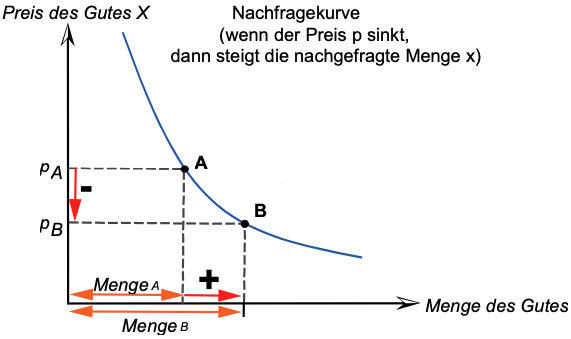
\includegraphics[width=7cm]{Typische_Nachfragefunktion.png}
\end{center}

\subsection{Ein Modell zu Konsumentscheidungen von Haushalten}

\subsubsection{Budgetrestriktion}

\textbf{Budgetrestriktion}: Summe der Ausgaben für zwei verschiedene Güter ($x_1p_1 + x_2p_2$) entsrpicht einem Budget $B$

\begin{align}
    B = x_1p_1 + x_2p_2 \\
    x_2 = \frac{B}{p_2} - x_1 \frac{p_1}{p_2}
\end{align}

Wie bereits erwähnt, ist der Nutzen eine lineare Kombination von preisen und Menge an Gütern, welche für eine Indifferenzkurve auf dem gleichen Niveau liegt die Gruppe oder Schar der Niveaulienen ergeben ein Nutzengebirge

\begin{equation}
    U = C x_1^a x_2^b
\end{equation}

mit $C$, $a$, $b$ Konstanten ($a,b =$ Bedeutung des Guts)

\subsubsection{Indifferenzkurven}

\textbf{Der Grenznutzen}: Ist die Ableitung einer Indifferenzkurve auf dem Niveau $U$ bezüglich $x_1$ und $x_2$ und ist immer positiv: 

\begin{equation}
    \frac{\partial U}{\partial x_1}, \frac{\partial U}{\partial x_2} > 0
\end{equation}

\textbf{Der Grenznutzen nimmt ab}. Der Nutzenzuwachs nimmt immer mehr ab mit zunehmenden Gütern einer Sorte (Es gitb eine Sättigung):

\begin{equation}
    \frac{\partial^2 U}{\partial x_1^2}, \frac{\partial^2 U}{\partial x_2^2} < 0
\end{equation}

Die Grenzrate der Substitution (GRS) misst die substituierbarkeit zweier Produkte und bestimmen die Form der Indifferenzkurve: 

\begin{equation}
   GRS =  \frac{GN_2}{GN_1} = \frac{dU/dx_2}{dU/dx_1}
\end{equation}

wobei perfekte Substitute bei $GRS = 1$ und perfekte Komplement bei $GRS = \pm \infty, 0$ 

\subsubsection{Der optimale Konsumpunkt}

\textbf{Der optimale Konsumpunkt}: Ist derjenige Punkt, wo sich Budgetrestriktion und Indifferenzkurve sich tangieren. Es ist dabei der maximale Nutzen bei gegebenem Budget. Die Steigung lautet hier $GRS$ bzw. $p_1/p_2$. Preisverhältnis = Grenzrate der Substitution/Grenznutzenverhältnis

\subsection{Von der optimalen Entscheidung zur individuellen Nachfragefunktion}

\begin{enumerate}
    \item Preis nimmt zu $\rightarrow$ Budgetrestriktion dreht sich 
    \item Es ergibt sich ein neues Nutzenniveau mit neuem Optimum
    \item Die nachgefragte Menge nimmt ab 
\end{enumerate}

Die Nachfragekurve zeigt die Zahlungsbereitschaft des Kosnumenten und kann auch als Funktion des Grenznutzens in Abhängigkeit von der Gütermenge interpretiert werden. Damit wird Nutzen und der marginale Nutzenzuwachs quantifizierbar und daher vergleichbar. 
Falls das Budget des Konsumenten sich ändert, oder seine Präferenzen sich änderen, kann verschiebt sich die Nachfragekurve nach oben oder nach unten. 

\begin{center}
    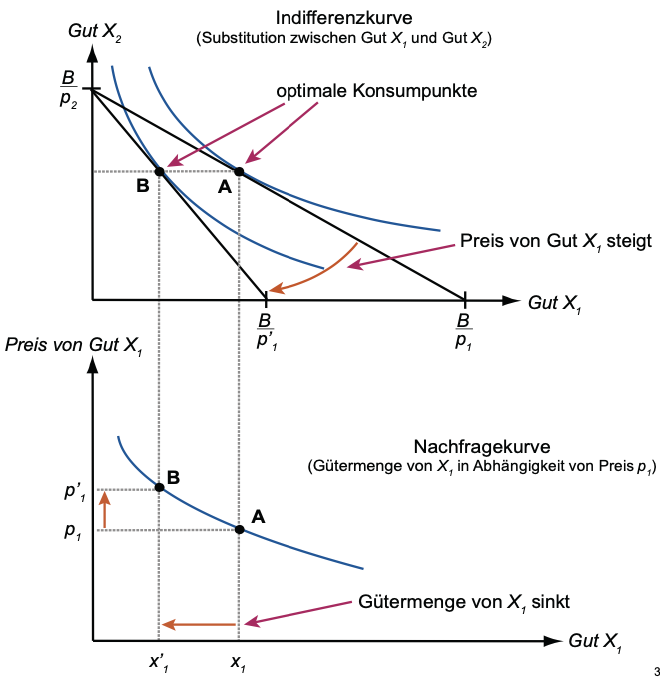
\includegraphics[width=7cm]{Nachfragefunktion.png}
\end{center}

\subsection{Preiselastizität der Nachfrage}

Die Preiselastizität der Nachfrage gibt an, um wie viel Prozent sich die nachgefragte Menge eines Gutes sich ändert als Folge einer einprozentigen Veränderung
des Preises dieses Gutes:

\begin{equation}
    \varepsilon_x N_p = \frac{\text{relative Mengenänderung}}{\text{relative Preisänderung}} = \frac{\frac{\Delta x^N}{x^N}}{\frac{\Delta p}{p}} = \frac{\Delta x^N}{\Delta p}\frac{p}{x^N}
\end{equation}

Im Grenzübergang $\Delta \rightarrow \partial$ beziehungsweise $\Delta p \rightarrow 0$:

\begin{equation}
    \varepsilon_x N_p = \frac{\partial x^N}{\partial p}\frac{p}{x^N}
\end{equation}

Die Preiselastizität hängt also von der Steigung der Nachfragekurve ($\frac{\partial x}{\partial p}$) und vom Preis/Mengenverhältnis ab. Entlang der Nachfragekurve variiert also die Elastizität. Da Nachfragekurven meist konvex sind, ist die die Preiselastizität negativ und nur der Betrag wird angegeben,
um das Ausmass zu repräsentieren. \newline \newline

Typen von Elastizität: 
    \begin{itemize}
        \item Vollkommen unelastisch ($\varepsilon = 0$): Preisänderung hat keinen Einfluss auf Nachfrage 
        \item Vollkommen elastisch ($\varepsilon = \pm \infty$): Preisänderung hat einen unendlichen grossen Einfluss auf Menge 
        \item Einheitselastisch ($\varepsilon = 1$): Preisänderung hat direkt gekoppelt mit Nachfrageverhalten 
        \item Elastisch ($\varepsilon > 1$): Die Nachfrage sinkt um mehr als ein Prozent wenn der Preis um 1 Prozent erhöht wird
        \item Unelastisch ($0<\varepsilon<1$): Die Nachfrage sinkt weniger als ein Prozent wenn der Preis um 1 Prozent erhöht wird
        \item Isoelastisch ($\varepsilon = const$): Die Nachfrage sinkt um einen konstanten Prozentsatz bei einer 1-prozentigen Erhöhung der Nachfrage
    \end{itemize}

Andere Arten der Elastizität: 

    \begin{enumerate}
        \item Einkommenselastizität der Nachfrage $\varepsilon_{x,Y}$: Veränderung der prozentualen Nachfragemenge eines Gutes $X$ aufgrund des veränderten Einkommens (Konsumbudget) $Y$. Diese ist meistens positiv (Konsum nimmt zu mit höherem Einkommen)
        \item Kreuzpreiselastizität $\eta_{x_1,p_2}$: Änderung der Nachfrage nach Produkt $X_1$ aufgrund er Preisänderung eines anderen Produkts $X_2$. Positive Kreuzpreiselastizitäten ergeben sich bei Substituten. Bei Komplementen ist die Kreuzpreiselastizität negativ 
    \end{enumerate}

\begin{align}
    \varepsilon_{x,Y} = \frac{\Delta x}{\Delta Y} \frac{Y}{x} \\
    \eta_{x_1,p_2} = \frac{\Delta x_1}{\Delta p_2}\frac{p_2}{x_1}
\end{align}

\section{Angebotsverhalten und Unternehmen}

\subsection{Güterangebot von Unternehmen bei volkommner Konkurrenz}

Zielvariable ist der Gewinn, der maximiert werden sollte. Randbedingungen: Güternachfrage und andere Unternehmen, die dasselbe Gut produzieren. Die Gewinnfunktion lautet (in Abhägnigkeit der Gütermenge $x$): 

\begin{equation}
    G(x) = E(x) - K(x) = px -K(x)=  \text{Erlös} - \text{Kosten}
\end{equation}

\begin{itemize}
    \item Notwendige Bedingung: $\frac{\partial G}{\partial x} = 0$ (Lok. Maximum / Minimum)
    \item Hinreichende Bedingung: $\frac{\partial^2 G}{\partial x^2} < 0$ (Negativ Gekrümmt)
\end{itemize}

Bei \textbf{Vollkommener Konkurrenz} gehen wir davon aus, dass einzelne Unternehmen keinen Einfluss auf den Preis haben. Wir bezeichnen den Preis $p$ als $\overline{p}$. Daraus folgt:

\begin{equation}
    \overline{p} = K' = \frac{\partial K}{\partial x} = E'
\end{equation}

\begin{itemize}
    \item $K'$: Grenzkosten: Gibt an, wieviel die zusätzlichen Kosten sind für jede weitere Produktion eines Gutes 
    \item $E'$: Grenzerlös: Zusätzlicher Erlös beim Verkauf jedes weiteren Gutes 
\end{itemize}

Die \textbf{Güterangebotsfunktion} ergibt sich, wenn man die Funktion $K'(x)$ explizit nach der Gütermenge auflöst:

\begin{equation}
    x^A = f(p),  \text{~mit } f'(p) > 0
\end{equation}

Die Grenzkostenkurve ist positiv steigend aufgrund der steigenden Kosten bei erhöhter Produktionsmenge. Die Kostenkurve ist in der Realität of durch eine S-förmige Kurve angenähert. Zuerst sinken die Grenzkosten (Kapazitätsauslastung steigt) und steigen nachher wieder an (Kapazitätsüberlastung) 

\begin{center}
    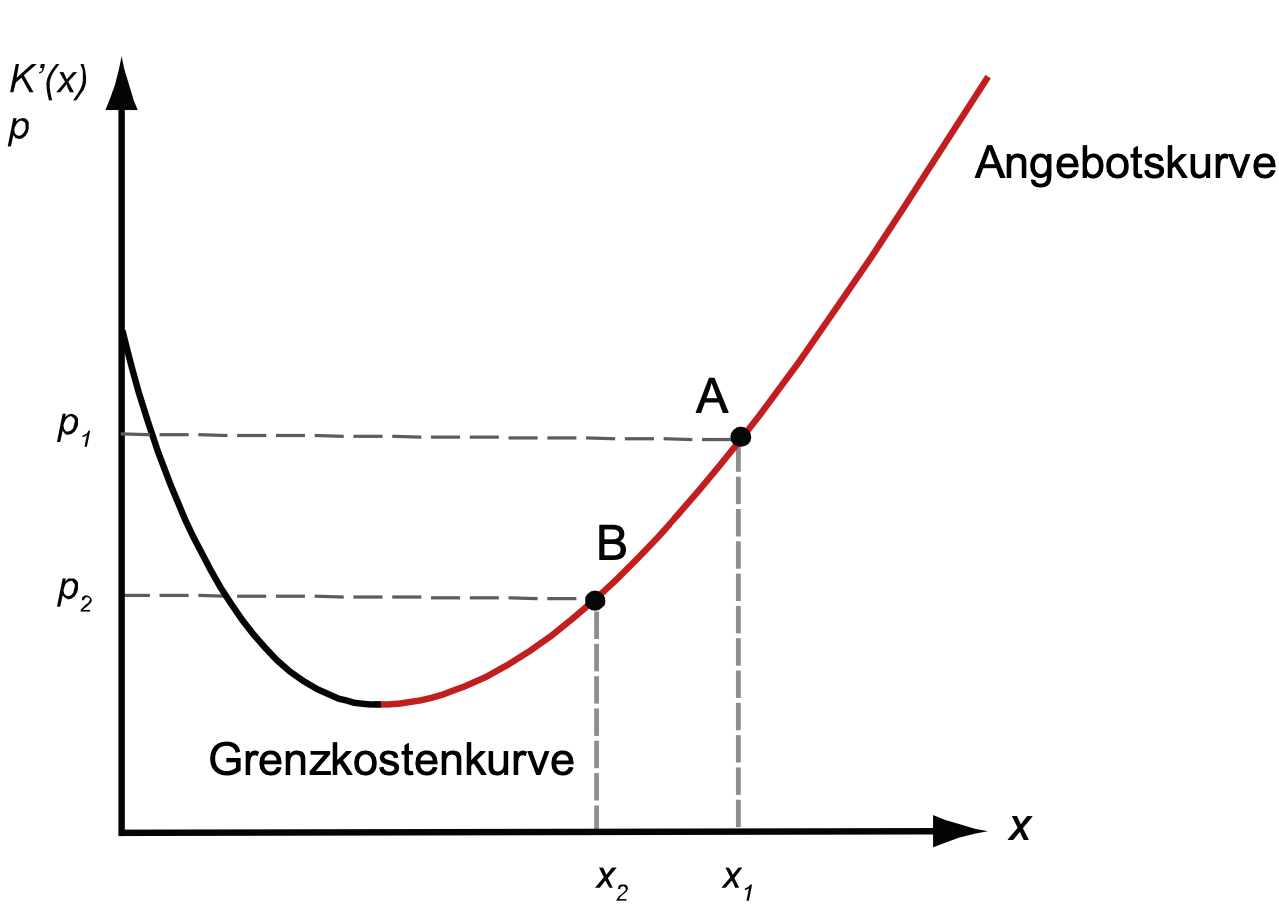
\includegraphics[width=6.5cm]{Gueterangebotsfunktion_Unternehmen.png}
\end{center}

\textbf{Kostenfunktion}: Abhängig von Fixkosten (von produzierten Menge unabhängig) und variable Kosten (von prod. Menge abhängig/steigen mit Produktionsmenge an). Die Grenzkosten sind unabhängig von den Fixkosten. Die Fixkosten bestimmen die Achsenverschiebung der Kostenfunktion. Die Kostenfunktion stellt den Zusammenhang zwischen Produktionsmenge und den jeweils minimalsten Kosten für $x$ dar.

\begin{equation}
    K(x) = K_{fix} + K_{var}(x)
\end{equation}

Die \textbf{Durchschnittkosten} $k$ beschreiben die Kosten pro Einheit:

\begin{equation}
    k(x) = K(x)/x
\end{equation}

Der \textbf{s-förmige Kostenverlauf}: Die Angebotskurve nimmt mit zunhemender Produktionsmenge nachdem die Grenzkosten erreicht worden sind zu. Bei Punkt $x_1$ sind die Kosten für jede weitere Produktion eines Gutes minimal. Die Steigung $\tan\alpha$ vom Ursprung aus ist dasselbe wie $k(x) = K(x)/x$ aus der Darstellung ersichtlich. Wenn man nun den Winkel in Abhängigkeit von $x$ plottet erhält man das Minimum der Durchschnittskostenkurve

\begin{center}
    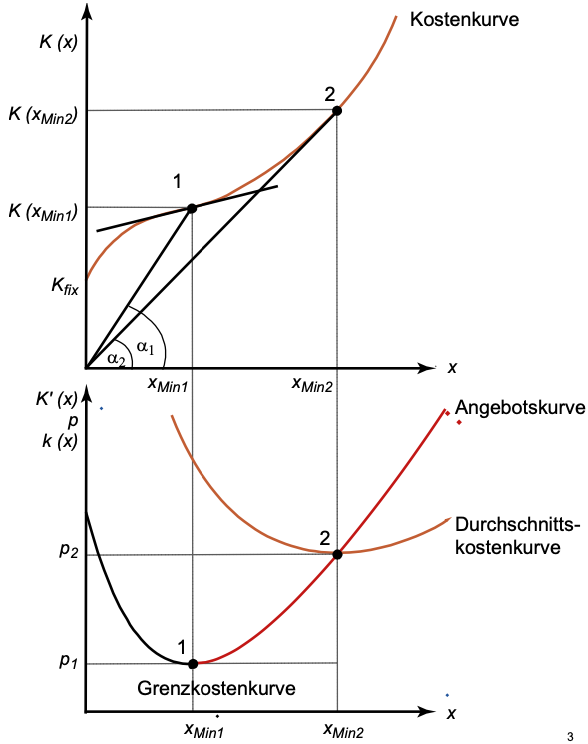
\includegraphics[width=8cm]{S-Foermiger-Kostenverlauf.png}
\end{center}

Die Produktionsfunktion bestimmt den s-förmigen Verlauf der Kostenfunktion. Mathematisch wird der Kostenverlauf folgendermassen definiert: 

\begin{equation}
    X = A a^\alpha k^\beta
\end{equation}

Wo $a$ die Arbeitsmenge und $k$ die Kapitalmenge repräsentieren. $A$, $\alpha$ und $\beta$ sind variable Parameter. 
Aufgrund der Form dieser Kurve (p. 5 / Kap. 3), kann man den Begriff der \textbf{Skalenerträge} definieren.Steigende Skalenerträge gehen mit fallenden Grenzkosten
bzw. langfristigen Durchschnittskosten einher. \newline \newline

\textbf{Langfristiges Betriebsminimum}: Ist der Ort, wo die Grenzkosten und die totalen Durchschnittskosten (TDK) gleich gross sind. Bei dieser Produktionsmenge sind die totalen Durchschnittskosten minimal und der Gewinn beträgt Null. \newline \newline
\textbf{Kurzfristiges Betriebsminimum}: Ist der Ort, wo die Angebotskurve die variablen Durchschnittskosten (VDK) schneiden (Firma möchte Fixkosten decken)

\begin{center}
    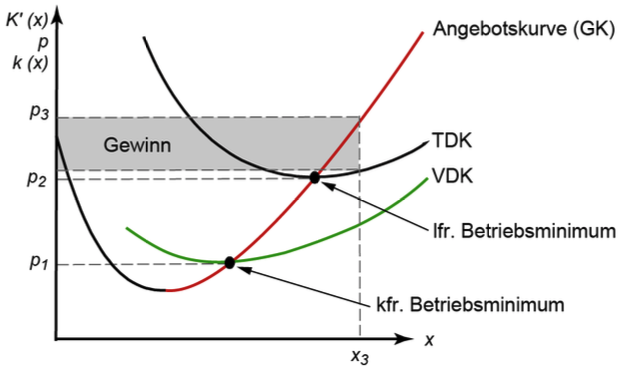
\includegraphics[width=7cm]{Betriebsminima.png}    
\end{center}



\subsection{Güterangebot eines Monopolisten}
\textbf{Monopol}: Ist eine Marktform, bei der es einen Anbieter und sehr viele, kleine Nachfrager gibt. Der Monopolist kann den Preis selbst bestimmen. Die zugehörige Menge wird bestimmt durch die Nachfragefunktion. Entstehungsgründe für ein Monopol:

\begin{itemize}
    \item Unternehmen hat Schlüsselressourcen, zu denen nur es Zugang hat (Diamanten z.B.)
    \item Wird vom Staat erschaffen, um einen Schlüsseldienst (Post) oder Urheberschutz gewährleistet wird (Bücher, Musik)
    \item Bei hohen Skalenerträgen, hohen Fixkosten und tiefen Grenzkosten. So lohnt es sich eher, dass nur eine Firma mit tieferen Durchschnittskosten besser produzieren kann als mehrere
\end{itemize}

Die Gewinnfunktion kann nun folgendermassen definiert werden und es gelten die gleichen Bedingungen wie bei vollständiger Konkurrenz, ausser dass nun der Preis $p(x)$ variabel ist:

\begin{align}
    G(x) = p(x) x - K(x) \\
    G'(x) = p'(x) x + p(x) 1 - K'(x) = 0\\
    G''(x) < 0 \Leftrightarrow K''(x) < p'(x)x + p(x)
\end{align}

Die Menge $x^*$, wo die notwendige und hinreichende Bedingung erfüllt ist, kann in die Nachfragefunktion eingesetzt werden ($p^* = p(x^*)$). Man nennt diesen Punkt \emph{Cournotpunkt}. Ändert sich die Nachfragekurve (Verschiebung, Drehung), so verändert sich die Lage des Cournotpunktes.



\subsection{Preiselastizität des Angebots}

Die \textbf{Preiselastizität des Angebots} gibt an, um wieviel Prozent sich die angebotene Menge eines Gutes verändert als Folge einer einprozentigen Veränderung des Preises dieses Gutes.

\begin{equation}
    \varepsilon_xA_p = \frac{\partial x^A}{\partial p}\frac{p}{x^A}
\end{equation}

Die Preiselastizität variiert in der Regel entlang der Kurve. Wir referenzieren $p$ und $x$ immer auf den Nominalwert (alten Wert)

\subsubsection{Verschiedene Elastizitätswerte}

Die Preiselastizität des Angebots ist meistens positiv aufgrund der Annahme, dass das Angebot mit steigendem Preis steigt. Falls:

\begin{itemize}
    \item $\epsilon_x A_p = 1$, dann geht die Angebotskurve durch den Ursprung
    \item $ \epsilon_x A_p > 1$, genau dann, wenn die Angebotskurve die Preisachse schneidet und ist undendlich bei $x^A = 0$ und konvergiert nach 1 für $x^A \rightarrow \infty$
\end{itemize}


\section{Kosten-Nutzen Analyse}

Grundlegendes Vorgehen: 

\begin{enumerate}
    \item Auflisten von Kosten und Nutzen über eine Laufzeit eines Projektes 
    \item Bestimmung des Nettonutzen pro Periode ($N_t-K_t$)
    \item Gewichtung der Nettonutzen nach zeitlichem Anfall (NPV)
    \item Auswahl: Handlungsalternative mit positiven NPV zu wählen oder andere Entscheidungskriterien
\end{enumerate}

\subsection{Gegenstand}
Grundidee: Systematische Gegenüberstellung von Kosten und Nutzen. Individuum wird eine Aktivität/Handlungsalternative x nur dann ausführen, wenn deren Kosten (costs) kleiner sind als deren Nutzen (benefits). Hierbei muss ebenfalls beachtet werden, dass es intagible 
Kosten gibt (nicht messbar) sowie mögliche Opportunitätskosten nicht berücksichtigt werden beim Assessment solcher Kosten. In der Volkswirtschaft wird dann diejenige Alternative berücksichtigt, welche der
Gesellschaft netto am Grössten Nutzen bringt. 

\begin{equation}
    \text{Max} \sum_{t=1}^T \delta^t(B_t - C_t),~ B_t = \sum_{i=1}^I B_{it}~\text{und}~ C_t = \sum_{i=1}^T C_{it}
\end{equation}

$B_i$ kann man interpretieren als die Zahlungsbereitschaft eines Individuums (max. bereit zu bezahlender Betrag), und $C_i$ für die Aktivität erforderlichen Aufwendungen.

\subsection{Bestimmung von Kosten und Nutzen}
Werden Güter auf (vollständigen) Märkten gehandelt, so entsprechen deren Preise der marginalen Zahlungsbereitschaft eines durchschnittlichen Individu- ums und determinieren die bereitgestellte (gehandelte) Gütermenge. Werden Güter nicht auf einem Markt gehandelt, sondern durch den Staat bereitgestellt, müssen Kosten und Nutzen der Bereitstellung anderweitig ermittelt werden. Während Kosten oft aufgrund von Kostenrechnungen bereits monetär erfasst werden, werden Nutzen (Opportunitätskosten) i.d.R. mit Hilfe der Zahlungsbereitschaft bewertet.
\subsubsection{Indirekte Methoden (Revealed Preference)}

\begin{itemize}
    \item Kompensationsmethode bei Schäden: Welcher Wert an Gütern muss eingesetzt werden, um Schäden zu ersetzen. Z.B. geringer Fischfang wegen Wasserverschmutzung. Reparaturkosten in Marktwerten ausdrücken. Anwendbarkeit nur bei reversiblen Schäden.
    \item Aufwandmethode/Reisekostenmethode: Die Kosten, die einem Individuum aus dem Besuch eines Ortes entstammen. Man fragt nach, wieviel eine Person aufgewandt hat um von seinem Herkunftsort an eine Destination zu gelangen. Alle Individuen können so zusammengefasst werden und die Daten sind vergleichbar 
    \item Hedonische Preise: Zahlungsbereitschaft für Güter mit ähnlichen Charakteristika (z.B. Immobilien an Ort X vs. Y). Wie ändert sich der Preis eines Hauses, wenn die Luftverschmutzung um 1\% zunimmt? Vorgehen: $Preis = f(Eigenschaften)$, erste Ableitung ist der hedonische Preis 
\end{itemize}

\subsubsection{Direkte Methoden (Stated Preference)}

\begin{itemize}
    \item Contingent Valuation: Hier werden Individuen mit einem Szenario konfrontiert und direkt über ihre Zahlungsbereitschaft (Willingness to Pay) befragt. Auf der anderen Seite werden Individuen gefragt, für wieviel Geld sie auf dasselbe Gut verzichten würden, der sogenannten Aktzeptantbereitschaft (Willingness to Accept). Oft gilt $WTP < WTA$
    \item Discrete Choice Experiment: Es werden Eigenschaften eines Guts definiert. Daraus lassen sich die Eigenschaften als Vektor definieren mit mehreren Dimensionen. Mehrere Alternativen an Gütern werden Individuen gezeigt und so kann statischtisch bestimmt werden, was die Zahlungsbereitschaft eines Guts ist.
\end{itemize}

\textbf{Zeitpräferenz}: Geld, dass man in der Zukunft erhält, und nicht jetzt, hat für ein Individuum weniger wert. Aus diesem Grund wir der sogenannte Diskontierungsfaktor $0 \leq \delta \leq 1$ definiert (siehe Gl. 21). \newline \newline

\textbf{Diskontrate vs. Marktzinssatz}: Die Diskontrate wird oft bestimmt via des Marktzinssatz $r$ bestimmt. Wir nehmen an, es gibt einen Zins auf den Betrag den man heute besitzt. Nach einem Jahr ist der Betrag $(1+r)$ wert. Also ist der aktuelle Diskontfaktor $\delta = 1/(1+r)$ .
Zusätzlich können andere, theoretische Überlegungen gemacht werden und die Diskontrate abhängig von der Gesellschaft modellieren: $\delta = z + ng$, wobei

\begin{itemize}
    \item $z$: Die pure Zeitpräferenz ist
    \item $n$: Der abnehmende Grenznutzen des Konsums, ausgedrückt durch die Einkommenselastizität des Konsums $n$
    \item $g$: Die Wachstumsrate des Pro-Kopf Konsums 
\end{itemize}



\subsection{Umgang mit Zeitkomponente}
\textbf{Barwertmethode und Net Present Value (NPV)}: 

\begin{equation}
    NPV = \sum_{t=0}^T \delta^t \left( N_t - K_t\right),~ N_0 = 0
\end{equation}

\textbf{Nutzen für zukünftige Generationen}: Hierbei ist zu beachten, dass es sich lohnt, zukünftige Einnahmen weniger abzudiskontieren. Der Nutzen ist langfristig angedacht und für zukünftige Generationen. Beispiel dafür sind Umwelthematiken. Hier kann man solche Projekte folgendermassen interpretieren: 

\begin{enumerate}
    \item Normale Diskontrate: Es handelt sich um ein Investitionsprojekt
    \item Tiefe Diskontrate: Weil sonst der Nutzen weggerechnet wird 
\end{enumerate}

\subsection{Unsicherheit}

\begin{itemize}
    \item Unsicherheit: Wir wissen nicht, mit welcher Wahrscheinlichkeit ein Ereignis auftritt
    \item Risiko: Es gibt Ereignisse oder Umweltzustände, über deren Eintreten wir nicht sicher sind aber wir kennen die Wahrscheinlichkeit (positives oder auch negatives Ereignis). Man kennt die objektive Wahrscheinlichkeit
    \item Ambiguität: Zwischenform von Unischerheit und Risiko. Der Entscheidungsträger entscheidet basierend auf subjektiver Wahrscheinlichkeit. 
    \item Erwartungswert: Werden für Risiken gemäss Statistik für Kosten wie auch Nutzen bestimmt $E(C) = \sum C_k p(C_k)$
    \item Risikoaversion: Viele Menschen würden anstatt auf den Erwartungswert immer eine sichere Alternative wählen. 
\end{itemize}


\subsection{Verteilungsproblematik}

\begin{itemize}
    \item Pareto-Effizienz: Grösstes Problem der Kosten-Nutzen-Analyse: Es sind keine Aussagen möglich, wie die Kosten und Nutzen innerhalb der Gesellschaft alloziert sind. Die Pareto-Effizienz ist ein Kriterium für die Einordnung der Verteilung
    \item Eine Güterverteilung gilt dann als effizient, wenn keine andere Güterverteilung möglich ist, welche mindestens ein Individuum besser, gleichzeitig aber kein anderes Individuum schlechter stellt 
    \item Gemäss K-N Analysen wird dann immer eine Massnahme empfohlen, wenn die Summe der Benefits die Summer der Kosten übersteigen, unabhängig von we die Kosten getragen werden. Diese Effizienz wird \emph{potentielle Pareto-Effizienz} genannt
    \item Die notwendige Bedingung für ein soziales Optimum (Pareto-Optimum) ist bei vollständigem Wettbewerb gegeben (Usage-Costs/Wohlfahrt-Kosten). Im Marktleichgewicht gilt Grenznutzen (Nachfrage) = Grenzkosten (Angebot)
\end{itemize}

\begin{equation}
    \max\limits_x\left\{U(x)-K(x)\right\} \Leftrightarrow U'(x) = K'(x)
\end{equation}

Es ist wichtig anzumerken, dass die Kosten-Nutzen Analyse gute Resultate bringen kann, jedoch müssen die Parameter offengelegt sein.
\section{Analyse von Märkten}

\subsection{Aggregierte Angebots- und Nachfragekurven}

Die Aggregation findet horizontal statt. Je mehr Akteure,umso glatter wird die Angebotskurve/Nachfragekurve

\begin{center}
    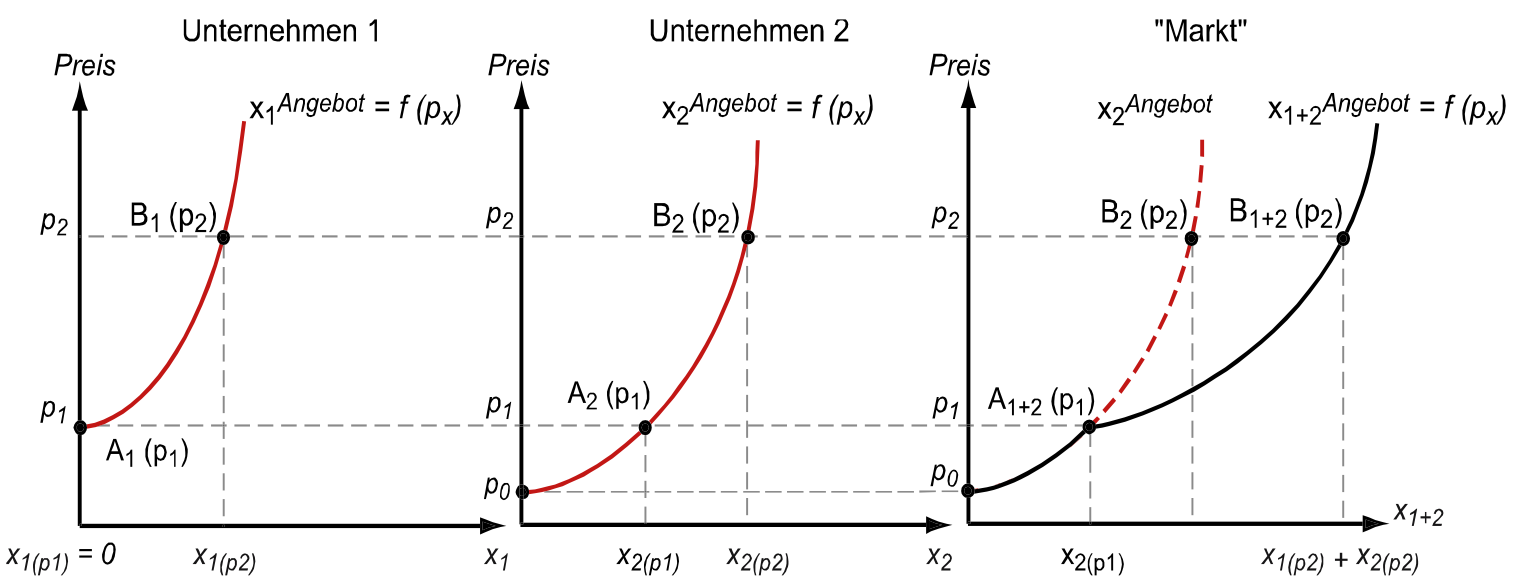
\includegraphics[width=8cm]{Angebotskurve_Aggregiert.png}
\end{center}

Hierbei ist zu beachten, dass die Mengen $x$ bei konstantem $p$ aufaddiert werden! Dies bedeutet, dass man zuerst die Gleichungen $x(p)$ aufstellen muss und dann aufaddiert.

\subsection{Preisbildung auf Märkten}

\subsubsection{Preisbildung bei vollkommener Konkurrenz}

Annahme: Markt besteht aus vielen, kleinen Unternehmen und wird von vielen kleinen Haushalten in Anspruch genommen. Die Unternehmen wie auch die Haushalte haben keinen Einfluss auf den Preis. Weitere Annahme: Die Funktionen für Nachfrage und Angebot sind bekannt.
Die angebotene Menge und nachgefragte Menge werden über den Marktpreis bestimmt. Der Marktpreis is so hoch, dass Marktpreis und Angebotspreis gleich hoch sind. 

\begin{center}
    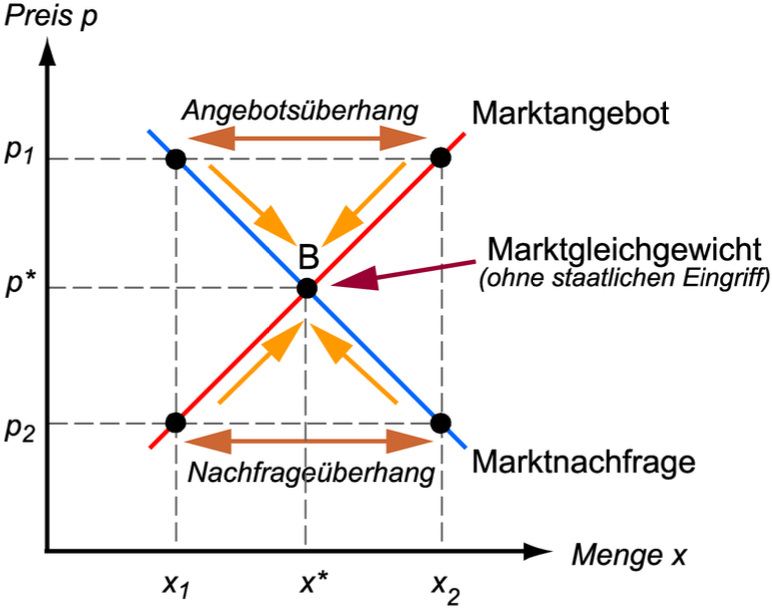
\includegraphics[width=5cm]{Marktgleichgewicht_1.png}
\end{center}

Bei $p_1$: \textbf{Angebotsüberhang} besteht nur kurzfristig. Das Marktangebot ist höher als die nachgefragte Menge. Andere Anbieter bieten allenfalls keine Produkte mehr an, da die Kosten unterhalb der Durchschnittskosten liegen\newline 

Bei $p_2$: \textbf{Nachfrageüberhang} besteht nur kurzfristig. Die Marktnachfrage ist höher als die angebotene Menge. Nachfrager ziehen sich aus dem Markt zurück oder verringern die nachgefragte Menge \newline 

Das \textbf{Marktgleichgewicht} liegt da, wo der Markt geräumt ist, d.h. der Preis gerade so hoch ist, dass Marktnachfrage und Angebot gleich hoch sind. Marktgleichgewichte bestehen nur kurzfristig, gegeben alle Informationen sind vorhanden und der Staat greift nich ein.
Die Anpassungen zum Preis zu gleich grossen Mengen finden sehr schnell statt. 


\subsubsection{Preisbildung beim Monopol}

Punkt $A$ ist der Cournot-Punkt. Er liegt auf der Nachfragekurve und bestimmt diejenige Preis-Mengen-Kombination (pMonopol,xMonopol), die für den Monopolisten gewinnmaximal ist. Im Punkt $B$ gilt, dass der Grenzerlös (aus der Nachfragekurve abgeleitet) den Grenzkosten (aus der Kostenkurve des Monopolisten abgeleitet) entspricht. Punkt $C$ ist derjenige Punkt, der bei vollkommener Konkurrenz dem Marktgleichgewicht entsprechen würde. Der Monopolpreis $p_{Monopol}$ ist höher als der Konkurrenzpreis $p^*$ und die Menge $x_{Monopol}$ ist geringer als die Konkurrenzmenge $x^*$. Es werden also in dieser Marktform einige Nachfrager ausgeschlossen bzw. einige Nachfrager können nicht soviel konsumieren wie es bei der Marktform der vollkommenen Konkurrenz der Fall wäre.

\begin{center}
    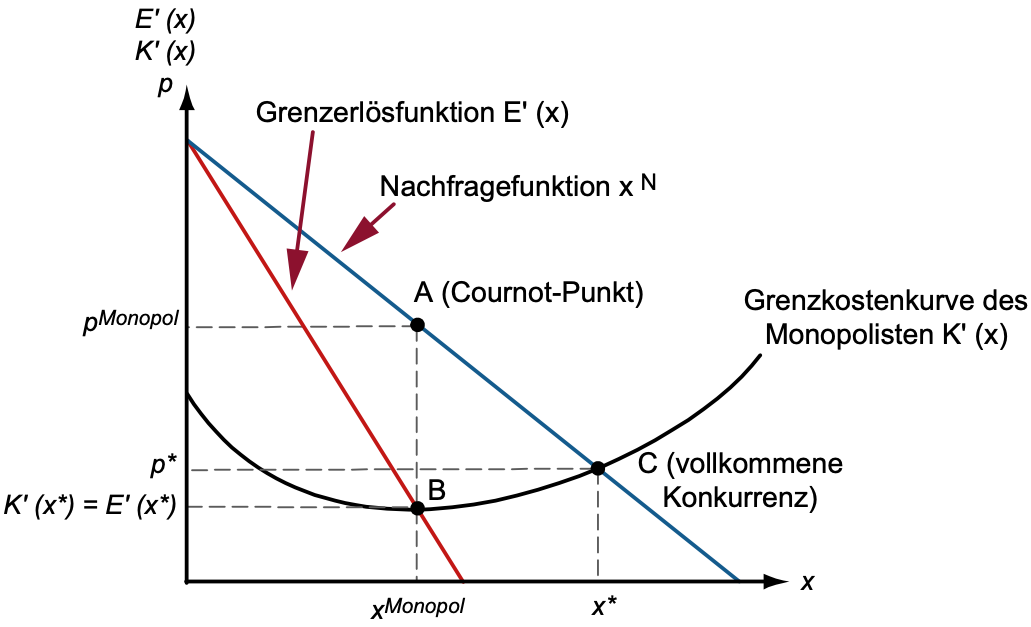
\includegraphics[width=7cm]{Preisbildung_Monopol.png}
\end{center}

Der Preis beim Monopol ist höher als bei der völligen Konkurrenz. Ebenso verringert sich die angebotene Menge. Argumente zugunsten Monopole sind:

\begin{itemize}
    \item Die Aussicht auf Gewinne/Monopole entwickeln Unternehmen neue Technologien, zur Senkung der Prodsuktionskosten und zur Verbesserung der Leistungen 
    \item Gewinne während einer gewissen Übergangsphase sind gut (benefit of monopoly)
    \item Forschungs- oder Entwicklungskosten können mittels Monopolgewinne amortisiert werden 
    \item Hierzu nötig sind jedoch geeignete Rahmenbedingungen: Klare Bedingungen zu den Verfügungsrechten und möglichst kleine Eingriffe in den Marktmechanismus selbst 
\end{itemize}

\subsubsection{Natürliches Monopol}

\textbf{Natürliche Monopole} sind gekennzeichnet durch: 

\begin{itemize}
    \item Sehr hohe Fixkosten (Hohe Investitionen nötig)
    \item Niedrige Grenzkosten 
    \item Durchschnittkosten, die wegen hohen Fixkosten über den Grenzkosten liegen 
\end{itemize}

Der Verkäufer würde somit einen Verlust schreiben mit jedem verkauften Stück. Bei der Kostenstruktur des natürlichen Monopols kommt es nicht zu einem Angebot konkurrierender Anbieter. 
Im Falle des Monopols ist es nämlich möglich, dass der Preis höher als die Durchschnittskosten und Grenzkosten ist. Ein derartiger hoher Monopolpreis ermöglicht dann zwar die Erstellung des jeweiligen Gutes mit steigenden Skalenerträgen, ist jedoch verbunden mit einer tiefen Verbrauchsmenge; eine solche Konstellation bringt Wohlfahrtsverluste mit sich.
Folgende Massnahmen bieten sich an: 

\begin{itemize}
    \item Staat produziert das Gut selbst 
    \item Staat legt einen Höchstpreis fest für den Monopolisten (mit vorbestimmten Erlös)
    \item ``Unbundling'': Netwerke (Gas-/Wasserleitungen) werden getrennt in Bereitstellung und Betrieb. Die Bereitstellung ist monopolistisch, während der Betrieb und die Ressourcen (Wasser, Öl) zu offiziellen Konditionen angeboten werden 
\end{itemize}

\begin{center}
    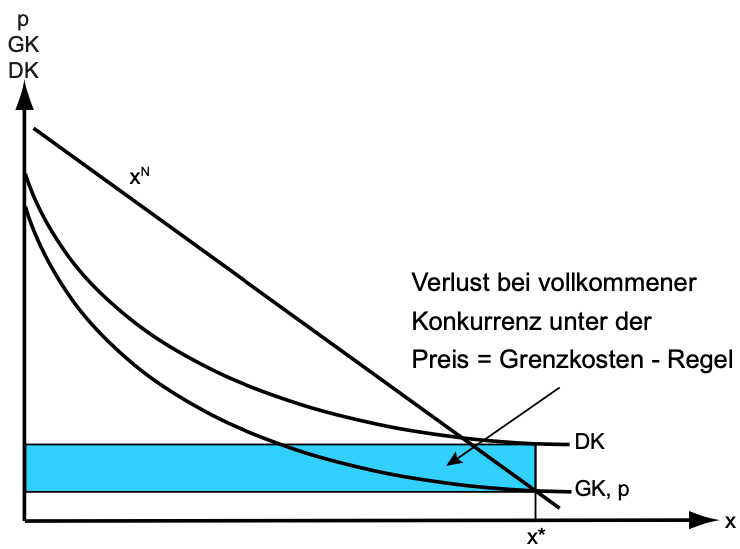
\includegraphics[width=5.5cm]{Natuerliches_Monopol_Preise.png}
\end{center}

Beim natürlichen Monopol kann sich die einfache Regel/Grenzkostenregel nicht angewandt werden. Der optimale Preis ist der Punkt, wo die Durchschnittskosten ($DK$) und Nachfragefunktion ($x^N$) sich schneiden

\subsection{Ökonomische Renten}

\subsubsection{Renten bei vollkommener Konkurrenz}

\textbf{Konsumentenrente}: Ist die nicht-ausgeschöpfte Zahlungsbereitschaft des Kunden. Geometrisch ist dies die Fläche unterhalb der Nachfragekurve, welche oberhalb des Marktpreises liegt. \newline

\textbf{Produzentenrente}: Erlöse - (variable) Kosten. Die Produzentenrente besteht aus den Erlösen ($p\cdot x$) ohne die Kosten für die Produktion ($\int K' dx$). \newline

Das Konzept der Produzentenrente impliziert dass Unternehmen in der Lage sind Gewinne zu machen. Dies ist in einem Modell der vollständigen Konkur- renz nur kurzfristig möglich. Langfristig führen Gewinnaussichten in einer Branche dazu, dass immer mehr Anbieter auf den Markt drängen. Dies führt zu einer Reduktion der Gewinne. Am Ende dieses Prozesses gehen (in einer solchen statischen Analyse) die Gewinne gegen null.

\begin{center}
    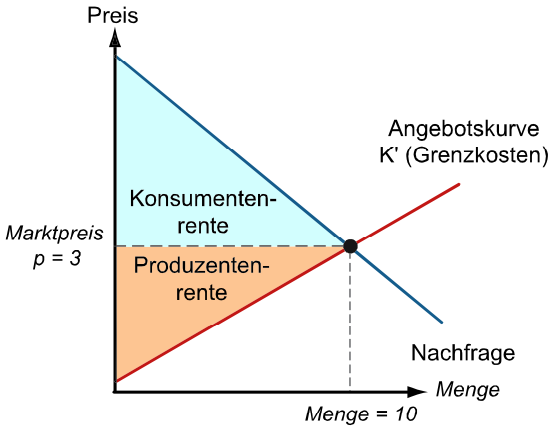
\includegraphics[width=6cm]{Rentenkonzept.png}
\end{center}

\subsubsection{Renten beim Monopol}

\textbf{Konsumentenrente}: Entspricht nun derjenigen Fläche, welche vom Cournotpunkt aus und der Nachfragefunktion eingeschlossen ist \newline \newline
\textbf{Produzentenrente}: Entspricht derjenigen Rente, welche zwischen Cournotpunkt und Angebotskurve/ Grenzkostenkurve liegt. \newline \newline
Im Vergleich zum vollkommenen Markt führt es einerseits zu einer Konvertierung der Konsumentenrente in Produzentenrente. Andererseits führt es auch zu einem sogenannten \textbf{Wohlfahrtsverlust}. Dieser ist beschränkt durch die verminderte Menge, die Verkauft werden kann. Die Konsumentenrente (D) sowie die Produzentenrente (I) nehmen genau um die Fläche ab, welche durch die verminderte Menge entsteht.

\begin{center}
    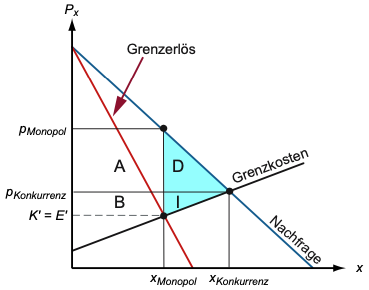
\includegraphics[width=6cm]{Wohlfahrtsverlust.png}
\end{center}

\subsection{Höchst- und Mindestpreise}
\subsubsection{Mindestpreise}

\begin{itemize}
    \item Motivation: Begünstigung von Produzenten (Versuch mittels höherer Preise Einkommen der Produzenten zu erhöhen) durch den Staat 
    \item Beispiele: Produkte der Landwirtschaft, Mindestlöhne
    \item Konsequenz: Angebotsüberhang
    \item Staatliche Reaktionsmöglichkeiten: Ankauf + Verwendung durch Staat oder Subventionierung der Nachfrager 
    \item Alternative: Kontingentierung (Maximum Output definieren)
\end{itemize}

\subsubsection{Höchstpreise}

\begin{itemize}
    \item Motivation: Begünstigung von Konsumenten (Versuch mittels tieferer Preise zur Verringerung der Ausgaben für ein bestimmtes Gut)
    \item Beispiele: Wohnungsmieten, Energiepreise für Entwicklungsländer
    \item Konsequenz: Nachfrageüberhang 
    \item Staatliche Reaktionsmöglichkeiten: Zuteilungsmechanismen (Ähnlich zu Kontingentierung), Subventionierung der Anbieter (Förderung von Wohnungsbau/Objektförderung)
    \item Alternative: Zweckgebunde Transfers an Nachfragegruppen (Subjektförderung)
\end{itemize}

\subsection{Verbrauchssteuern}

Ver- brauchssteuern werden erhoben, wenn bzw. weil der Staat Einnahmen erzie- len will (fiskalische Funktion) und wenn bzw. weil der Verbrauch eines besteu- erten Gutes gesenkt werden soll, wie z.B. aus ökologischen oder gesundheit- lichen Gründen (Lenkungsfunktion).
Eine Verbrauchssteuer ist ein Aufschlag auf den Marktpreis, der entweder pro Mengeneinheit (Mengensteuer) oder pro Werteinheit (Wertsteuer) berechnet werden kann. Bei der Mengensteuer wird ein fixer Geldbetrag pro Einheit auf den Preis aufgeschlagen. Bei der Wertsteuer wird ein bestimmter Prozentsatz auf den Preis des Gutes aufgeschlagen.

\begin{itemize}
    \item Die Verbrauchsteuern verschieben die Angebotskurve nach oben. Der Preis erhöht sich direkt um den Wert der Steuer $t$
    \item Die nachgefragte Menge geht zurück
    \item Der Umsatz nimmt ab. Der Produzent kann nur mit der neuen nachgefragten Menge und den gleichbleiben Grenzkosten rechnen. Die Produktion geht zurück.
\end{itemize}

Die Steuerlast wird folgendermassen aufgeteilt (Konsument = D, Produzent = E):

\begin{center}
    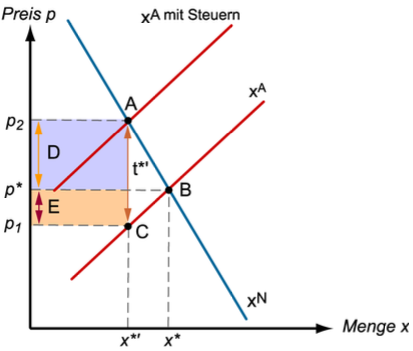
\includegraphics[width=5cm]{Steuerlast.png}
\end{center}

\subsection{Subventionen}

Subventionen haben zwei Hauptziele:

\begin{itemize}
    \item Umsätze von Produzenten sollen steigen oder auf hohem Niveau (Sicherung von Arbeitsplätzen)
    \item Preise, zu denen der Nachfrager kaufen kann, sollen sinken, sodass die Nachfrage steigt (ÖV)
    \item Die Kosten trägt der Staat
\end{itemize}

\begin{center}
    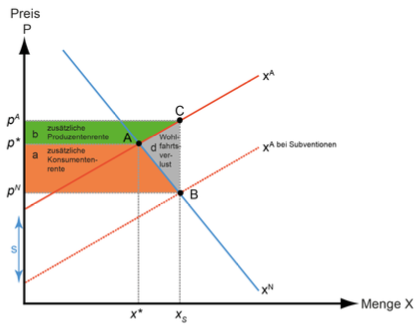
\includegraphics[width=7cm]{Subventionen.png}
\end{center}

Die Angebotskurve verschiebt sich nach unten um den Preis $s$. Die Menge steigt an. Dies führt zu einem neuen Gleichgewichtspreis bei $B$. Beachte, dass die Produzentenrente $b$ nun oberhalb der Konsumentenrente $a$ sich befindet.

\section{Öffentliche Güter und externe Effekte}

\subsection{Öffentliche Güter}

\begin{itemize}
    \item Öffentliche Güter sind durch Nicht-Ausschliessbarkeit und Nicht-Rivalität im Konsum gekennzeichnet 
    \item \textbf{Nicht-Ausschliessbarkeit} vom Konsum bedeutet, dass niemand vom Konsum eines Guts ausgeschlossen werden kann
    \item \textbf{Nicht-Rivalität} im Konsum bedeutet, dass der Konsum eines Guts durch ein Individuum keine Konsequenzen auf den Konsum des Guts durch andere In- dividuen hat.
    \item Wegen Nicht-Ausschliessbarkeit im Konsum kann es zum Trittbrettfahrerproblem kommen (ähnlich zu Prisoner's Dilemma), wobei es zu einer Unterversorgung der öffentlichen Güter kommen kann
    \item Trittbrettfahrerproblem sind Probleme, wobei eine Person den Mitnutzer wird eines Gutes, ohne dafür bezahlen zu müssen. Lösung: Staatliches Angebot oder staatliche Vorschriften, falls private kein Angebot machen können
    \item Ein anderes Problem wäre auch, dass es zu einer Übernutzung von Gütern und Ressourcen kommen könnte. Lösung hierzu: Vergabe von Nutzungsrechten oder Einführung von Preisen
    \item Das Soziale Optimum kann nicht erreicht werden, wenn das Indiviuum den Eigennutz maximieren möchte 
\end{itemize}

\begin{center}
    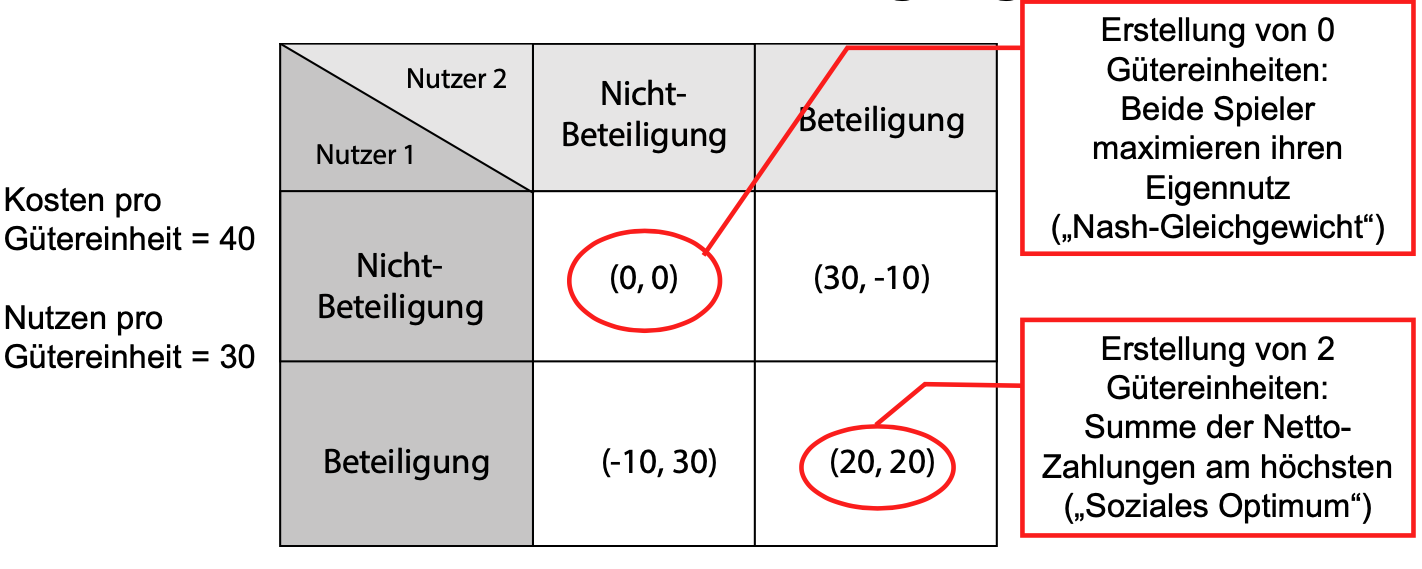
\includegraphics[width=7cm]{Oeffentliche_Gueter_Auszahlungsmatrix.png}
\end{center}

\begin{center}
    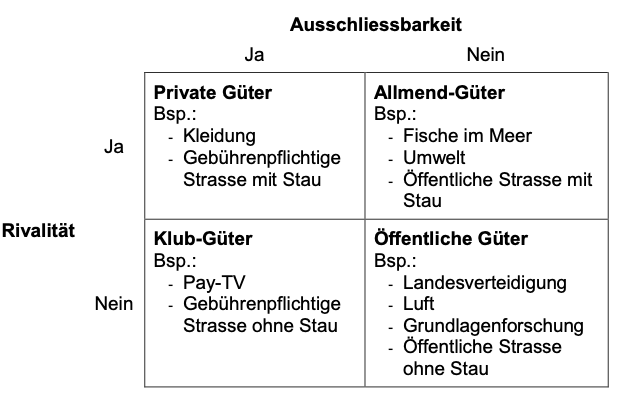
\includegraphics[width=7cm]{Typen_von_Guetern.png}
\end{center}



\subsection{Externe Effekte}

Effekte welche ausserhalb des Preissystems einer Volkswirtschaft anfallen, werden als Externalitäten oder externe Effekte bezeichnet. Diese können einen positiven wie auch negativen Einfluss auf die Produzenten wie auch Konsumenten haben.

\begin{itemize}
    \item Negativer externer Effekt auf die Produktionsmöglichkeiten Dritter: Schadstoffe von Firma A beinflussen die Produktion von Firma B
    \item Negativer externer Effekt auf die Konsummöglichkeiten Dritter: Schadstoffe von Firma A beeinflussen die Umwelt von Konsumenten C
    \item Positiver externer Effekt auf die Produktionsmöglichkeiten Dritter : Symbiose - Firma A produziert Produkt a, und Firma B produziert Produkt b. a und b werden bessser.
    \item Positiver externer Effekt auf die Konsummöglichkeiten Dritter: Konsument A konsumiert etwas, wovon Konsument B profitiert
\end{itemize}

Negative und positive externe Effekte beeinträchtigen die Allokations-Effizienz einer Gesellschaft. Die Preise für die verschiedenen Güter sind falsch in dem Sinn, dass sie nicht die wahren Knappheitsverhältnisse widerspiegeln. \newline 

Fallen externe Kosten an, sind die Grenzkosten für die Gesellschaft grösser als die Grenzkosten für das einzelne Individuum. Der Marktpreis für das Gut ist dann aus gesellschaftlicher Perspektive zu tief und die verbrauchte Menge zu hoch. \newline

\textbf{Soziale Grenzkosten} bezeichnen die wahren Grenzkosten einer Handlung und nicht nur denjenigen Teil, wel- cher unmittelbar bei produzierenden Firmen anfällt (private Grenzkos- ten). Die sozialen Grenzkosten entsprechen der Summe aus den privaten Grenzkosten und den gesellschaftlichen Zusatzkosten einer bestimmten Handlung. \newline

\textbf{Sozialer Grenznutzen}: Gesellschaftliche oder soziale Grenznutzen bezeichnen die wahren Grenznutzen einer Handlung und nicht nur denjenigen Teil, der unmittelbar bei den Konsumierenden anfällt. Die sozialen Grenznutzen entsprechen der Summe aus den privaten Grenznutzen und dem gesell- schaftlichen Zusatznutzen einer bestimmten Handlung. \newline 

Der Impact von \textbf{Sozialem Zusatznutzen} kann interpretiert werden als eine Verschiebung der Nachfragekurve nach oben = negative externe Effekte

\begin{center}
    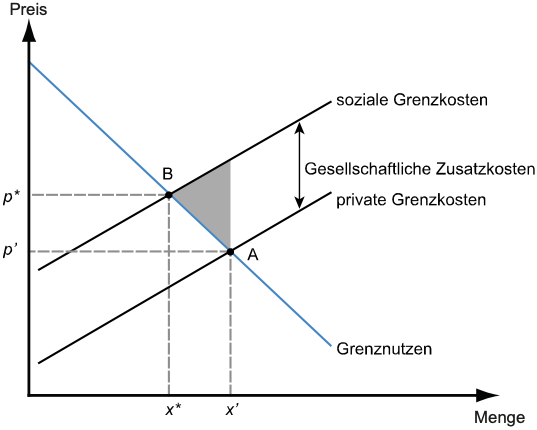
\includegraphics[width=7cm]{Negative_Effekte.png}
\end{center}

\begin{center}
    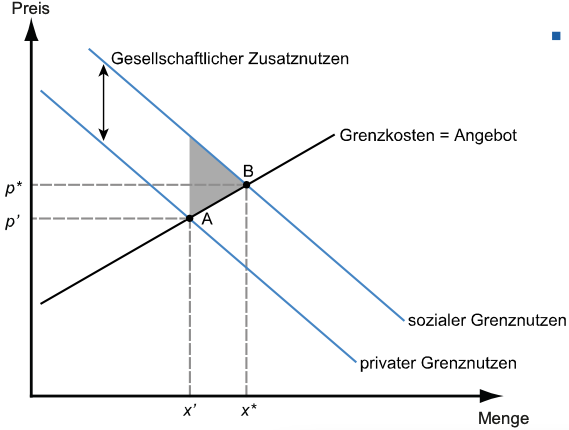
\includegraphics[width=7cm]{Positive_Effekte.png}
\end{center}

Der Impact von \textbf{Sozialen Zusatzkosten} kann interpretiert werden als eine Verschiebung der Angebotkurve nach oben  \newline 

Es kommt zu einem Wohlfahrtsverlust in beiden Fällen für die Gesellschaft 

\subsection{Internalisierung externer Effekte}

Um Wohlfahrtsverluste zu vermeiden, werden staatliche Eingriffe angeschaut: \newline

\textbf{Coase-Theorem}: Durchsetzung von Eigentums- und Nutzungsrechten (weniger starke Methode)

\begin{itemize}
    \item Verursacherprinizip: Eigentumsrechte bei Geschädigten. Verursacher des Schadens zahlt der Verursacher (Schadensersatz), da der Geschädigte aufgrund externer Effekte nicht produzieren oder konsumieren.
    \item Geschädigterprinzip: Eigentumsrechte beim Verursacher des Schadens. Der Geschädigte zahlt dem Verursacher eine Kompensation weil er einen Schaden vermeiden will. (Zur Sicherheit zahlt der Geschädigte für eine Sicherheit am Anfang)
\end{itemize}



\begin{center}
    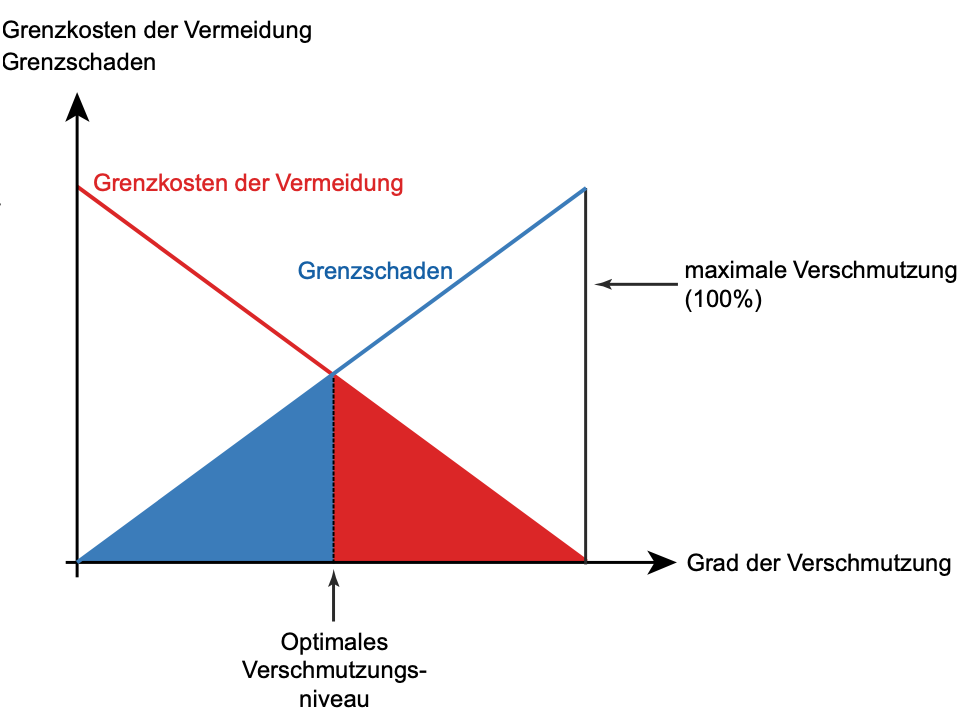
\includegraphics[width=7cm]{Coarse_Modell.png}
\end{center}



\textbf{Nachteile vom Coase-Theorem}:

\begin{itemize}
    \item Unvollständige Informtation: Werden alle Betroffenen berücksichtigt? Was sind die wahren Kosten?
    \item Eher geringe Relevanz auf nationaler Ebene, jedoch auf internationaler Ebene (Keine Weltregierung vorhanden)
    \item Asymmetrische Information: Sind alle Informationen für alle Reakteure zugänglich? Welches strategische Verhalten wenden Vertragspartner an?
    \item Transaktionskosten: Kontrollkosten möglich. Verhandlungen können so lange gehen, ohne dass ein Resultat daraus fruchtet.
    \item Verhandlungsmacht: Im Modell nicht berücksichtigt. Spielt eine wichtige Rolle für das optimale ökonomische Ergebnis 
\end{itemize}

\textbf{Pigou-Steuer / Starke Methode}: Grenzkosten durch Steuer so weit erheben, dass sie den gesellschaftlichen Grenzkosten entsprechen (Individuelle Grenzkostenkurve = Gesellschaftliche Grenzkostenkurve). Bei wenig preiselastischer Nachfrage kann kaum eine Mengenverringerung erreicht werden \newline 

\textbf{Preis-Standard-Ansatz}: Um eine gute Pigou-Steuer zu definieren, sollte man einen Preis-Standard $t$ zwischen individuellen und gesellschaftlichen Grenzkosten definieren

\begin{center}
    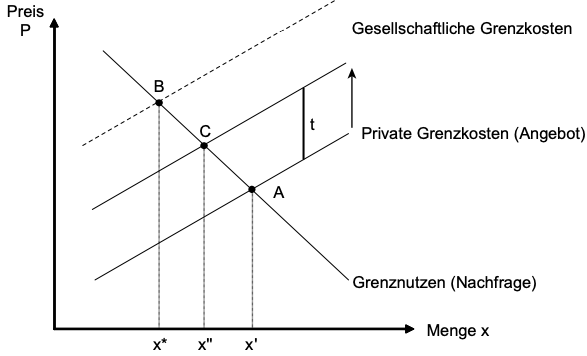
\includegraphics[width=7cm]{Preis-Standard-Ansatz.png}
\end{center}

\textbf{Mengenauflagen}: Anstatt einen Preis-Standard zu setzen, kann man es auch via Mengen kontrollieren. Hier werden maximal zulässige Grenzwerte definiert (z.B. Schadstoffmaxima). Bei negativen externen Effekten sind die Preise tendenziell zu tief und die Verbrauchsmengen zu hoch

\begin{center}
    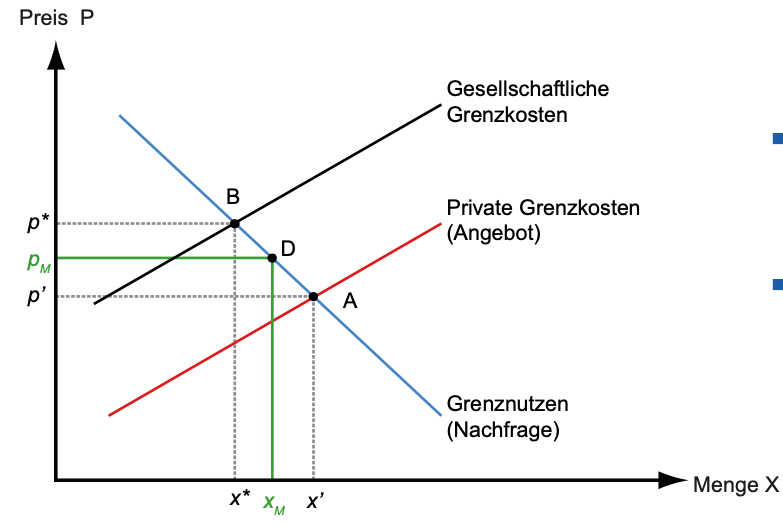
\includegraphics[width=7cm]{Mengenregulierung.png}
\end{center}

\textbf{Zertifikate}: Mengenauflagen können erreicht werden, in dem man Zertifikate festlegt wo eine Firma für ihre Mengen bezahlt und verhandeln kann, wieviele Emissionen möglich sind. Die Zertifikate sind auch handelbar. \\

\textbf{Beurteilungsmethoden verschiedener Internalisierungsmethoden}:

\begin{itemize}
    \item Ökologische Effizienz / Treffsicherheit
    \item Ökonomische Effizienz
    \item Implementierungskosten 
    \item Dynamische Anreizwirkungen
\end{itemize}

\textbf{Vergleich von Internalisierungsmethoden}

\begin{itemize}
    \item Mengenauflagen gelten als ökologisch wirksam
    \item Hauptnachteil von Auflagen: Ökonomisch ineffizient
    \item Steuern sind ökonomisch effizient
    \item Die Kosten für die Einführung von Steuern/Auflagen sind etwa je gleich hoch 
    \item Auflagen und Steuern setzen eine dynamische Anziehungswirkung
    \item Bei der Internalisierung positiver externer Effekte geht es vor allem darum, die Nachfrager zu einem höheren Verbrauch eines Gutes zu bringen
\end{itemize}

\section{Verhaltensökonomie}



\subsection{Homo Oeconomicus und Verhaltensökonomie}

Die Ökonomie versteht unter einem Homo Oeconomicus einen Akteur, der vor einer (ökonomischen) Entscheidung:

\begin{itemize}
    \item ...vollständig über alle möglichen Alternativen informiert ist 
    \item ...klare und stabile Präferenzen über all diese vielen Alternativen hat
    \item ...diejenige Alternative wählt, die seinen Präferenzen am besten entspricht (Nutzenmaximierung)
\end{itemize}

Entscheidungen eines Homo Oeconomicus werden als rational bezeichnet. Das Bild eines rein egoistischen, voll informierten, nutzenmaximierenden Menschen wurde schon früh als sehr restriktiv und wenig realistisch kritisiert. Dieser Kritik kann man aber entgegenhalten, dass Modelle, die mit den Homo Oeconomicus Annahmen arbeiten, in der Regel nicht das tatsächlich beobachtbare Verhalten einzelner Akteure erklären wollen, sondern zum Ziel haben, das Verhalten einer grossen Zahl von Akteuren im Durchschnitt zu beschreiben. 



\subsection{Heuristiken}

Menschen entscheiden sich häufig anhand einfacher Daumenregeln und analysieren nicht alle Handlungsmöglichkeiten. Folgende drei klassische Heuristiken existieren:

\begin{itemize}
    \item Verankerung: Von Vielzahl von Informationen sticht ein konkretes Merkmal hervor 
    \item Vollständigkeit: Wir tendieren dazu, Aktivitäten die begonnen worden sind, zu komplettieren 
    \item Verfügbarkeit: Phänomene oder Erinnerungen bestimmen unsere Entscheidungen 
\end{itemize}

\subsection{Framing-Effekte}

Menschen ändern ihre Präferenzen je nach Formulierung des Entscheidungsproblems. Dies bedeutet nichts anderes, als dass sich die Präferenzordnung über eine gegebene Menge an Handlungsalternativen je nach framing ändert.



\subsection{Die Rolle anderer Individuen}

Wie schon erwähnt, scheint die Annahme, Individuen würden nur auf ihren eigenen (Konsum-) Nutzen achten, nicht zutreffend zu sein und zu falschen Prognosen zu führen. \\ \newline 
Der unmittelbare ökonomische Nutzen für die Individuen zählt, sondern auch der Nutzen aus den sozialen Beziehungen zu anderen. Im Ultimatum-Spiel scheint es dabei vor allem um Präferenzen für Fairness zu gehen, die den Teilnehmenden des Spiels wichtig sind, was vom Spieler, der die Aufteilung vornimmt, antizipiert wird.

\subsection{Berücksichtigung der Zeitperspektive}

Wir gingen davon aus, dass Entscheidungen und Konsequenzen von Entscheidungen im selben Moment eintreten, was eine wenig realistische und zu fehlerhaften Prognosen führende Annahme ist. Deshalb soll nun ein Auseinanderfallen vom Entscheidungszeitpunkt und den Konsequenzen und damit auch Unsicherheit über die künftigen Konsequenzen heutiger Entscheidungen explizit berücksichtigt werden. Die drei Arten von Unsicherheit sind:

\begin{itemize}
    \item Risiko: Man kennt präzise Wahrscheinlichkeiten für das Eintreten der künftigen
    Konsequenzen
    \item Ambiguität: Man kennt verschiedene mögliche Wahrscheinlichkeitsverteilungen für
    die künftigen Konsequenzen
    \item Unsicherheit: Man weiss nichts darüber, welche künftigen Konsequenzen eher als
    andere eintreten werden 
\end{itemize}

\textbf{Rationales Risiko-Modell:}

Anders als beim umgangssprachlichen Risikobegriff bezieht sich der ökonomische Risikobegriff nicht nur auf mögliche Schadensereignisse, sondern generell auf mögliche positive und negative Folgen unseres Handelns, die mit bekannten Wahrscheinlichkeiten eintreten. Es wird dann weiter davon ausgegangen, dass die Individuen durch Risikopräferenzen gekennzeichnet sind, welche durch Nutzenfunktionen u abbildbar sind. Die möglichen Folgen unserer Handlungen werden als Lotterien dargestellt:

\begin{align}
    L_j = L(a_j) = \left\{ x_{1j}, p_{1j};...;x_{nj},p_{nj}\right\} \\ 
    j_{opt} = \max\limits_j \left\{ p_{1j}u(x_{1j})+...+p_{nj}u(x_{nj})\right\} 
\end{align}

mit $a_j=$ Handlungen ($j$-verschiedene) und $x_{nj}$ Konsequenzen ($n$-verschiedene) mit jeweiligen Zutreffwahrscheinlichkeiten $p_{nj}$. Man möchte den Erwartungsnutzen maximieren. Das rationale Modell ist jedoch nur deskriptiv und kann nicht für eine Prognose hinzugezogen werden.  \\ \newline

\textbf{Prospect Theory = Neue Erwartungsnutzentheorie}: Man führt eine Bewertungsfunktion $v$ für Gewinne und Verluste ein (siehe Grafik) ein und eine gewichtete Wahrscheinlichkeitsfunktion $w(p)$. Grund dafür ist für $v$ die subjektive Empfindung von Wahrscheinlichkeiten.

\begin{center}
    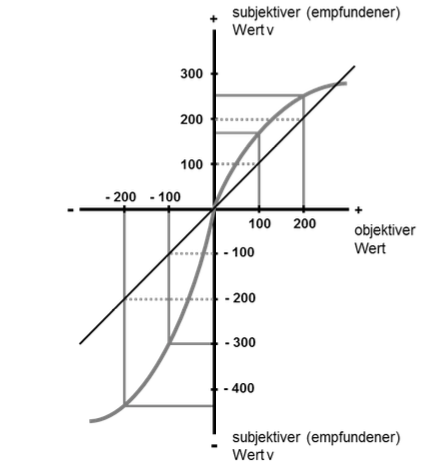
\includegraphics[width=5.5cm]{Bewertung_von_Gewinn_u_Verlust.png}
\end{center}

Unter Berücksichtigung von $v$ und $w$, ändert sich deas rationale Risiko-Modell:

\begin{equation}
    j_{opt} = \max\limits_j\left[ w(p_{1j})v(x_{1j})+...+w(p_{nj})v(x_{nj})\right]
\end{equation}

\subsection{Paradoxa}

\textbf{Allais-Paradoxon}: Man geht lieber mit einem sicheren Gewinn weiter als dass man versucht, gemäss Erwartungsnutzen zu entscheiden 

\textbf{Triell (Triple-Duell)}: Offenbar sind wir nicht gut in der Lage Wahrscheinlichkeiten für künftige Konsequenzen von Handlungen abzuschätzen, wenn die erforderlichen Kalküle komplexer und zeitaufwändiger sind. Wir lassen uns dann, ähnlich wie schon im Fall der Sicherheit, von einfachen Informationen am Anfang in die Irre führen und entscheiden uns daher nicht rational.

\subsection{Anwendungsbeispiel: Energienachfrage}

\begin{itemize}
    \item \textbf{Energy Efficiency Gap}: Energieeffizente Geräte werden eher nicht gekauft, obwohle es ökonomischer wäre 
    \item \textbf{Ökonomisch rationales Kalkül}: Differenz Anschaffungspreis und laufende Kosten 
    \item \textbf{Erklärung}
        \begin{itemize}
            \item Unwissen bezüglich Energieverbrauch
            \item Unkenntis über Kosten-Nutzen-Analyse 
            \item Kein Langfristendenken 
            \item Psychologische Effekte bei Informationsverarbeitung (Festhalten Status Quo)
        \end{itemize}
    \item \textbf{Möglichkeiten zum Abbau des Energy Efficiency Gap}:
        \begin{itemize}
            \item Erhöhung Strompreis
            \item Verbesserung der Information und auch Fähigkeit der Verbraucher, Information bearbeiten zu können
            \item Nudges/Schubser und soziale Netwerke/Medien 
            \item Zulassungen von Geräten mit höherer Effizienz 
        \end{itemize}    
\end{itemize}

\subsection{Fazit}

Die Verhaltensökonomie hilft, wirtschaftspolitische Empfehlungen abzuleiten, die sich an tatsächlich beobachtbarem Verhalten bzw. an tatsächlich beobachtbaren Entscheidungen von Individuen orientieren.

\section{Leistungskraft und Wohlfahrt von Ökonomien}

\subsection{Nationale Buchhaltung und Bruttoinlandprodukt}

\begin{itemize}
    \item Nationale Buchhaltung: Datenbasis für wirtschaftliche Leistungsfähigkeit einer Volkswirtschaft
    \item Sozialprodukt: Indikator für die Leistungsfähigkeit der Wohlfahrt von Volkswirtschaften
\end{itemize}

In der Makroökonomie werden die ökonomisch Transaktionen zwischen den Akteuren als geschlossene Kreisläufe angenommen. Der erweiterte Wirtschaftkreislauf berücksichtigt folgende Interaktionen:

\begin{itemize}
    \item Staat-Haushalte: Löhne, Steuern, Sozialtransfers
    \item Staat-Unternehmen: Steuern, Subventionen, Güterkäufe
    \item Unternehmen-Ausland: Exporte, Importe (Waren und Dienstleistungen)
    \item Unternehmen-Haushalte: Einkommen, Waren und Dienstleistungen, Produktionsfaktoren
\end{itemize}

Das \textbf{Sozialprodukt} (SP) ist der Wert aller während eines Jahres produzierten Gütern und Dienstleistungen. Es kann auf verschiedene Arten berechnet werden: \newline

\begin{tabular}{| c | c |}
    \hline 
    \textbf{Inlandsprodukt} & \textbf{Inländerprodukt} \\
    (Wert aller Güter und & (Wert aller Güter und \\
    Dienstleistungen, & Dienstleistungen,\\
    die im Inland produziert & die von den Inländern \\
    werden, inkl. von Ausländern) & produziert werden)\\
    \hline
    \textbf{Bruttoinlandprodukt (BIP)} & \textbf{Bruttosozialprodukt (BSP)} \\
    (Gross Domestic Product/GDP) & (Gross National Product/GNP) \\
    \hline
\end{tabular} \newline

Die Zusammenhänge zwischen den einzelnen Indikatoren sind in der folgenden Graphik ersichtlich:

\begin{tabular*}{8.1cm}{| l  l |}
    \hline
     & \textbf{Wert der produzierenten Waren und Dienst-}\\
     & \textbf{leistungen während einer Periode} \\
     $-$ & Vorleistungen \\
     + & Nichabzugfähige Mehrwertsteuer \\
     + & Nettoeinfuhrabgaben \\
     = & \textbf{Bruttoinlandprodukt zu Marktpreisen (BIP)} \\
     \hline
    + & Kapital- und Arbeitseinkommen der übrigen Welt \\
    $-$ & Kapital- und Arbeitseinkommen an die übrige Welt \\
    = & \textbf{Bruttoinländerprodukt zu Marktpreisen (BSP)} \\
    \hline 
    $-$ & Abschreibungen \\ 
    = & \textbf{Nettoinländerprodukt zu Marktpreisen} \\
    \hline
    + & Subventionen \\
    $-$ & Verbrauchssteuern und Einfuhrabgaben \\ 
    = & \textbf{Nettoinländerprodukt zu Faktorkosten} \\
     \hline
\end{tabular*} \newline \newline \newline

\textbf{Vorleistungen}: Vorleistungen werden vor jedem Wertschöpfungsschritt gemacht und müssen in der totalen Abrechnung Ganzen abgezogen werden, damit keine Doppelrechnungen entstehen \\ \newline

\textbf{Brutto vs. Netto}: Unterschieden zwischen Brutto- und Nettoinländerprodukte sind Abschreibungen, welche durch den Werteverzehr an Maschinen, Produktionsanlagen etc. während einer Periode auftritt \newline \newline

\textbf{Problem}: Abschreibungen beziehen sich nur auf Sachkapital und nicht andere Formen (Naturkapital z.B.) \newline \newline

\textbf{Marktpreise vs. Faktorkosten}: Beim Sozialprodukt werden alle Güter und Dienstleistungen inklusive ihren Steuern und Subventionen miteingerechnet. Die Knappheit der Güter werden daher durch staatliche Instrumente verzerrt. Um nur mit Faktorkosten zu rechnen, muss man diese inkludierten Instrumente ebenfalls abziehen. \newline \newline 

\textbf{Kaufkraftkorrekturen}: Die Kaufkraft des Dollars kann von Land zu Land unterschiedlich sein. Um die Kaufkraft zu berücksichtigen, werden \emph{Purchasing Power Parity Korrektoren} gemacht. Es wird also berechnet, wieviel in einen Warenkorb gelegt werden kann mit einem USD in einem Land und so erhalten Entwicklungsländer einen etwas höheres BIP wobei Industrieländer eine Senkung ihres BIP wahrnehmen.

\subsubsection{Erfassungsarten des BIP}

\begin{enumerate}
    \item Entstehungsrechnung/Produktionsansatz: Wert aller Waren und Dienstleistungen in einem Jahr. Hierbei werden alle Umsätze zusammengefasst
    \item Verwendungsrechnung: Hierbei wird vor allem auf den Konsum und die Investitionen Rücksicht genommen von Privathaushalten (Konsumenten), Staat (Staatsausgaben), vom Ausland (Export-Import) und Unternhemen (Investitionen). Die Ersparnisse der Haushalte werden mit den Investitionen aufgefangen (Kredit durch Bank an Unternhemen als Investition ursprünglich aus de Ersparnissen der Privathaushalte)
    \item Verteilungsrechung: BIP wird auf verschiedene Gruppen verteilt: Entweder nach Funktion (Produktionsfaktoren, Arbeit, Boden, Kapital) oder nach Person
\end{enumerate}

\subsection{Wohlfahrtmessung durch das Pro-Kopf Einkommen}

Die Wohlfahrtmessung nach Pro-Kopf Einkommen hat folgende Schwächen:

\begin{itemize}
    \item Nicht-Berücksichtigung von aussermarktlichen Leistungen: Eigenproduktion der Haushalte werden nicht berücksicht (Hausarbeit), unbezahlte Arbeiten und Freiwilligenarbeit
    \item Nicht-Berücksichtigung der Schattenwirtschaft: Arbeit, die den Ämtern nicht gemeldet werden
    \item Kontra-Intuitive Effekte: Gesundheitswesen, Naturkatastrophen, Umweltschäden/Unfälle. Wir errichten BIP-steigernde Massnahmen für solche Dinge und erhöhen das BIP, jedoch sind diese nicht zwingend wohlfahrtsteigend (Es geht mir nicht besser umbedingt wenn die Wirtschaft mehr Verkehrsunfälle bzw. Reparaturen macht)
    \item Qualitative/Immaterielle Askpekte nicht berücksichtigt: Sicherheit, Menschenrechte, Soziale Integration, Meinungsfreiheit, Zufriedenheit der Bevölkerung
    \item Personelle Einkommensverteilung der privaten Haushalte: Disparität von Einkommen im Land (Amzahl reiche und arme Menschen)
\end{itemize}

\begin{center}
    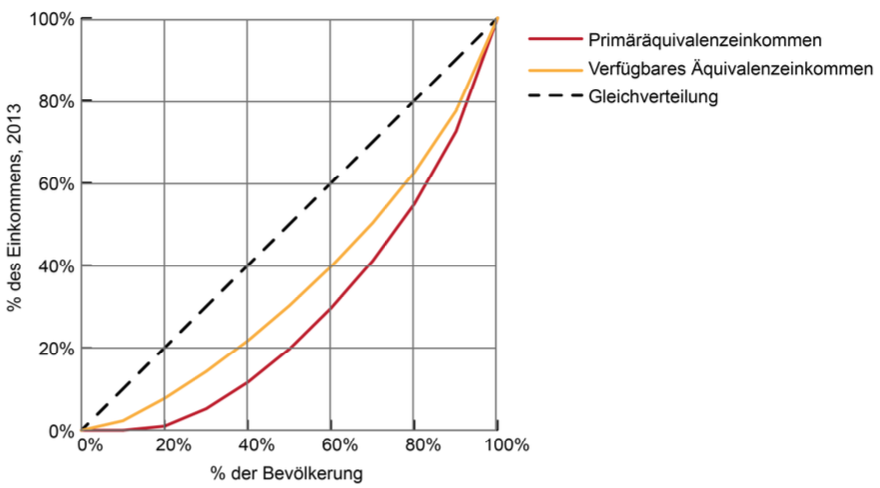
\includegraphics[width=8cm]{Lorenzkurve.png}
\end{center}

Die Lorenzkurve beschreibt die Einkommensverteilung der privaten Haushalte, dargestellt durch die Graphik. Auf der Ordinate abgetragen ist die Prozentzahl des aufsummierten Einkommens, wobei man ablesen kann dass eine Prozentzahl der Bevölkerung auf ein gewisses Einkommen Zugriff hat. Das Primäreinkommen ist das Einkommen ohne staatliche Umverteilung gerechnet. \newline \newline

\textbf{Gini Koeffizient}: Indikator für die Einkommensverteilung der Lorenzkurve und ist beschrieben durch Verhältnis von zwei Grössen. Einerseits durch denjenigen Teil der Kurve, welcher beschränkt ist durch die Gleichverteilung und der Lorenzkurve, andererseits auch durch die Gleichverteilung selbst.

\begin{itemize}
    \item Gini-Koeffizient $G=\frac{A}{A+B}$
    \item $G = 0$ genau wenn $A=0$: Lorenzkurve ist die Gleichverteilung - Einkommen perfekt gleichverteilt 
    \item $G=1$ genau wenn $A=A+B$: Lorenzkurve ist so stark nicht Gleichverteilt, dass das Einkommen vollständig bei einem Bruchteil (1\%) der Bevölkerung liegt. 
\end{itemize}

\textbf{Einkommensungleichheit}: Top 1\% tendiert höheres Einkommen zu haben \newline \newline

\textbf{Vermögenskonzentration}:Neben Unterschieden in der Einkommensverteilung gibt es auch unterschiedliche Vermögensverteilung. \newline \newline

\textbf{Fazit zu BIP}

Die Aussagekraft des BIP pro Kopf als Wohlstandsindikator ist eher gering. Es ist allerdings möglich, Indikatoren zu verwenden, die die oben geschilderten wohlfahrtsrelevanten Aspekte, welche nicht in das BIP eingehen, zusätzlich berücksichtigen. Die Gewichtung der einzelnen Indikatoren macht dann jedoch Werturteile erforderlich.Will man nur grobe Wohlfahrtsvergleiche zwischen Ländern machen, kann das BIP/Kopf allerdings trotz allem einen ersten Eindruck geben. Ein Vorteil des BIP/Kopf besteht im Übrigen auch darin, dass nahezu alle Länder weltweit ohne Zusatzkosten über die erforderlichen Daten verfügen.

\subsection{Determinanten des Pro-Kopf Einkommen}

Bei der Betrachtung des realen BIP der Schweiz sind zwei Phänomene zu beobachten:

\begin{enumerate}
    \item In der langen Frist steigt das BIP
    \item In der kurzen und mittleren Frist schwankt das BIP (Konjunkturschwankungen, siehe Bild)
\end{enumerate}

\begin{center}
    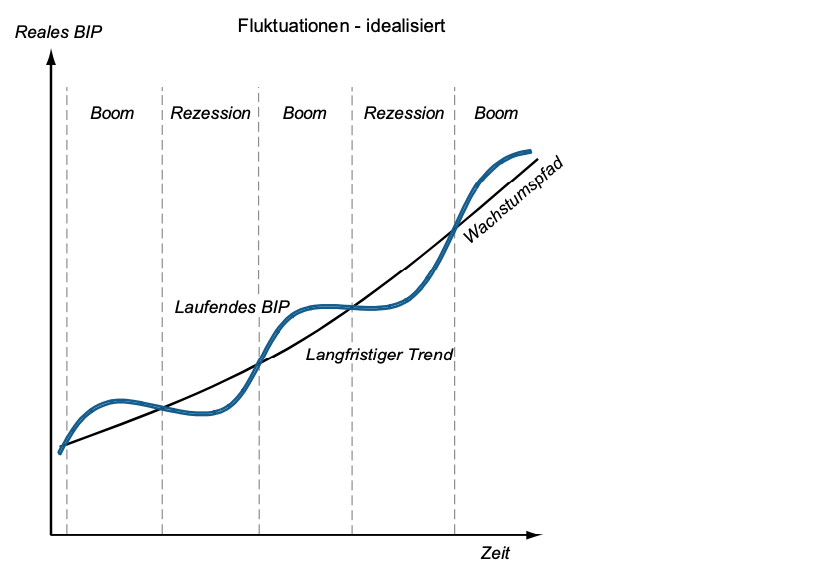
\includegraphics[width=9cm]{Konjunkurschwankungen_idealisiert.png}
\end{center}

\subsubsection{Wachstumsdeterminanten}

Gründe, warum ein positives Wirtschaftswachstum wünschenswert ist: 

\begin{enumerate}
    \item Materielle Versorgung der Menschen (wichtig für Entwicklungsländer): Entwicklungsländer profitieren vom Wachstum von Industrieländer einerseits durch Entwicklungszusammenarbeit, andererseits durch Märkte welche offen sind
    \item Umverteilung: Bei Wachstum ist die Umverteilung auf eine gleichmässigere Einkommensverteilung eher möglich. Wachstum ist notwendig, aber nicht hinreichende Bedingung für Umverteilung
    \item Zusätzliche Arbeitsplätze: Wachstum schafft neue Arbeitsplätze, gegeben Leute können umgeschult werden. Somit können weltweit auch die Kostenvorteile besser genutzt werden
\end{enumerate}

\begin{center}
    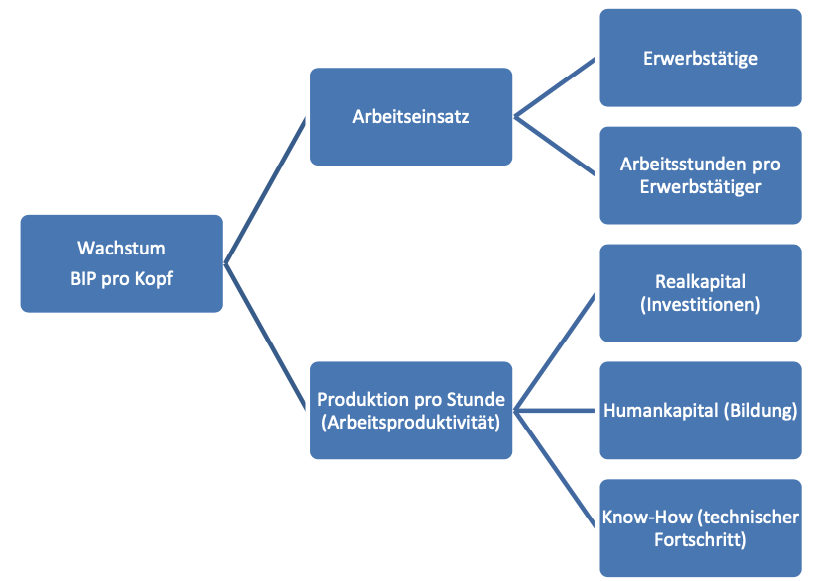
\includegraphics[width=8cm]{Wachstumsdeterminanten.png}
\end{center}

\subsubsection{Konjunkturdeterminanten}

Frage im Zusammenhang von Konjunkturzyklen:

\begin{itemize}
    \item Theoretisch: Ursachen für flache und steile Konjunkturzyklen?
    \item Wirtschaftpolitisch: Was kann man tun, um Zyklen möglichst lang und flach zu halten, damit die Anpassungskosten der Ökonomie minimal sind?
\end{itemize}

Die Werkzeuge der Wirtschaftspolitik zur Einflussnahme auf die Gesamtnachfrage sind wie folgt:

\begin{itemize}
    \item Direkte zusätzliche oder verringerte Staatsausgaben, zur kurzfristigen Erhöhung oder Senkung des BIP 
    \item Einflussnahem auf Konsum und Investitionen: Einkommenssteuern erhöhen oder senken, Zinsen für Investitionen erhöhen oder senken 
\end{itemize}

\subsection{Multiplikatoranalyse}

Ein mathematisches Modell, welche sich auf die vorhergehenden Faktoren stützt:

\begin{enumerate}
\item Gesamtnachfrage $Y^N$: 
    \begin{itemize}
        \item $Y^N = C+ I + A^{St} + (X-M)$
        \item $C ~\text{Konsumausgaben Private}$
        \item $I ~\text{Investitionen}$
        \item $A^{St}~\text{Staatsausgaben, Inv. und Konsum}$
        \item $X-M ~ \text{Leistungsbilanz (Aussenbeitrag)}  $
    \end{itemize}
\item Gesamtangebot: $Y^A$
\item Gleichgewicht am Gütermarkt: $Y^A = Y = Y^N$
\item Bestimmung der Konsumausgaben: \\ \\ $C = cY + C^{\text{autonom}}$ 
    \begin{itemize}
        \item $c$ marginale Konsumquote
        \item $C^{\text{autonom}}$ autonomer Konsum
    \end{itemize}
\end{enumerate}

\textbf{Multiplikatorprozess bei Staatsausgaben}: 

\begin{align}
    \Delta Y = \frac{1}{1-c} \Delta A^{St}, ~\Delta t = t_1-t_0 \\
    \text{Multiplikator} = \frac{1}{1-c}
\end{align}

Eine Erhöhung der Staatsausgaben erhöht die Gesamtnachfrage und somit auch das Volkseinkommen um den Betrag $\Delta A^{St}$. Dadurch werden selbstverstärkende Kreislaufmechanismen ausgelöst, die dafür sorgen, dass der Gesamteffekt grösser ist als der zusätzliche Ausgabenbetrag. \newline

\textbf{Steuer-Multiplikator}: 

\begin{align}
    \Delta Y = \frac{-c}{1-c} \Delta T \\
    \text{Multiplikator} = \frac{-c}{1-c}
\end{align}

Eine Senkung der Steuern erhöht das Sozialprodukt, und zwar um mehr als den ursprünglichen Steuersenkungsbetrag $ |\Delta T|$. \newline

\textbf{Vergleich von Steuer- und Staatsausgaben}:Steuermultiplikator ist kleiner als bei Staatsausgaben. Dies ist darauf zurückzuführen, dass eine Steuersenkung (-erhöhung) nicht unmittelbar in voller Höhe nachfragewirksam wird, sondern nur mittelbar über eine Erhöhung der privaten Konsumausgaben. Die Staatsausgabenerhöhung wirkt hingegen direkt. \newline 

\textbf{Multiplikator über steuerfinanzierte Staatsausgaben (Haavelmo Theorem)}

Es wird im folgenden angenommen, dass der Staat ein Steueraufkommen von T erzielt, mit welchem Staatsausgaben in Höhe von ASt finanziert werden: 

\begin{align}
    A^{St} = T \\
    \Delta Y = \frac{1}{1-c} \Delta A^{St} - \frac{c}{1-c} \Delta T \\
    \Delta Y = 1\cdot \Delta A^{St} \\
    \text{Multiplikator} = 1
\end{align}

Bei einer steuerfinanzierten Erhöhung der Staatsausgaben erhöht/vermindert sich das Volkseinkommen genau um den Betrag der Staatsausgaben (Haavelmo Effekt)

\subsection{Fiskalpolitik}

Unter Fiskalpolitik versteht man alle an Staatsausgaben oder Steuern ansetzenden Massnahmen des Staates, mit denen die konjunkturelle Entwicklung beeinflusst, d.h. gefördert oder gebremst werden soll.

\begin{itemize}
    \item Massnahmen vergleichsweise schnell im Vergleich zu Geldpolik
    \item Kritisch: "Crowding Out" - private Investitionen verringern sich als Reaktion durch Erhöhung durch Zinsen, welche durch die Kreditaufnahme des Staates herbeigeführt wurden
\end{itemize}

\section{Arbeitslosigkeit}

\subsection{Definition und Messung}

Gemäss SECO (arbeitslos): 

\begin{itemize}
    \item bei einem Arbeitsamt registriert
    \item gegenwärtig ohne Arbeit, arbeitet weniger als 6 Stunden pro Woche 
    \item innerhalb von 30 Tagen vermittlungsunfähig
\end{itemize}

\begin{equation}
    SECO = \frac{\text{registrierte (eingeschriebene) Arbeitslose}}{\text{Erwerbspersonen gemäss Volkszählung}}
\end{equation}

Gemäss BFS/SAKE (erwerbslos, ähnlich zu internationaler Standard):

\begin{itemize}
    \item in einer Referenzwoche weniger als 1 Stunde erwerbstätig waren
    \item in den vorangegangenen Wochen aktiv eine Arbeit gesucht haben 
    \item innerhalb von 4 Wochen mit einer Tätigkeit beginnen können 
\end{itemize}

\begin{equation}
    SAKE/BFS = \frac{\text{Erwerbslose}}{\text{Erwerbspersonen jährlich (Q3)}}
\end{equation}

Je nachdem, welches Mess-Konzept verwendet wird, fällt die Zahl der „Arbeitslosen“ bzw. „Erwerbslosen“ unterschiedlich hoch aus.

\subsection{Ursachen und Bekämpfung}

Will man Arbeitslosigkeit erklären, bezieht man sich i.d.R. auf einen Vergleich von gesamtwirtschaftlichem Arbeitsangebot und gesamtwirtschaftlicher Arbeitsnachfrage. Damit ist folgendes unterstellt:

\begin{itemize}
    \item Arbeit ist homogen, d.h. aus Vereinfachungsgründen sind Art und Qualität ausgeklammert 
    \item Arbeit wird von Firmen nachgefragt (Nachfragekurve)
    \item Arbeit wird von Personen angeboten (Angebotkurve)
\end{itemize}

Hierbei ist zu beachten, dass nun mikroökonomische Prinzipien wieder angewandt werden können

\subsubsection{Arbeitsangebot}

Wie bereits erwähnt, \emph{bieten die Arbeitnehmer Arbeit an} \newline 

Herleitung:

\begin{enumerate}
    \item Haushalt sieht Nutzen ($U$) in Freizeit ($f$) und Güterkonsum ($x$) $U = g(f,x)$
    \item Es sind maximal 18 Stunden Erwerbszeit möglich pro Tag (6 Ruhezeit). 
    \item Es folgt folgende Funktion:
    \begin{itemize}
        \item $f = 18-\frac{p}{w}x$
        \item Wobei es eine Budgetrestriktion gibt mit $xp =$ Warenkorb und $aw$ Entlöhnung (mit maximum 18 Stunden Arbeitszeit/Freizeit, $a$ Arbeitszeit und $w$ Lohn pro Zeit)
    \end{itemize}
    \item Das Optimum lässt sich finden als die Tangente, wo die maximale Nutzungsfunktion tangiert werden kann unter Berücksichtigung des Budgets
\end{enumerate}

\begin{center}
    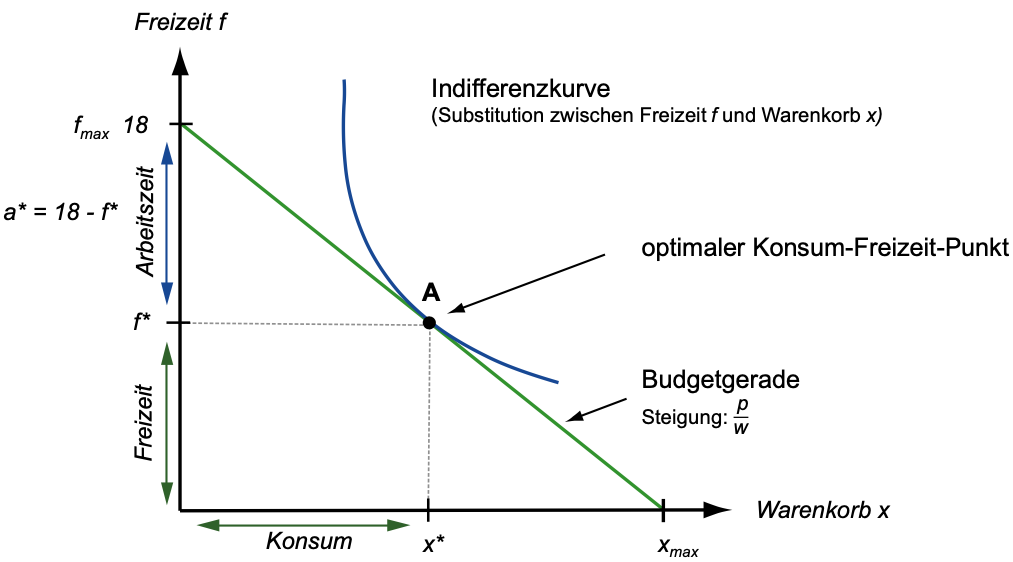
\includegraphics[width=8cm]{Arbeitsangebot.png}
    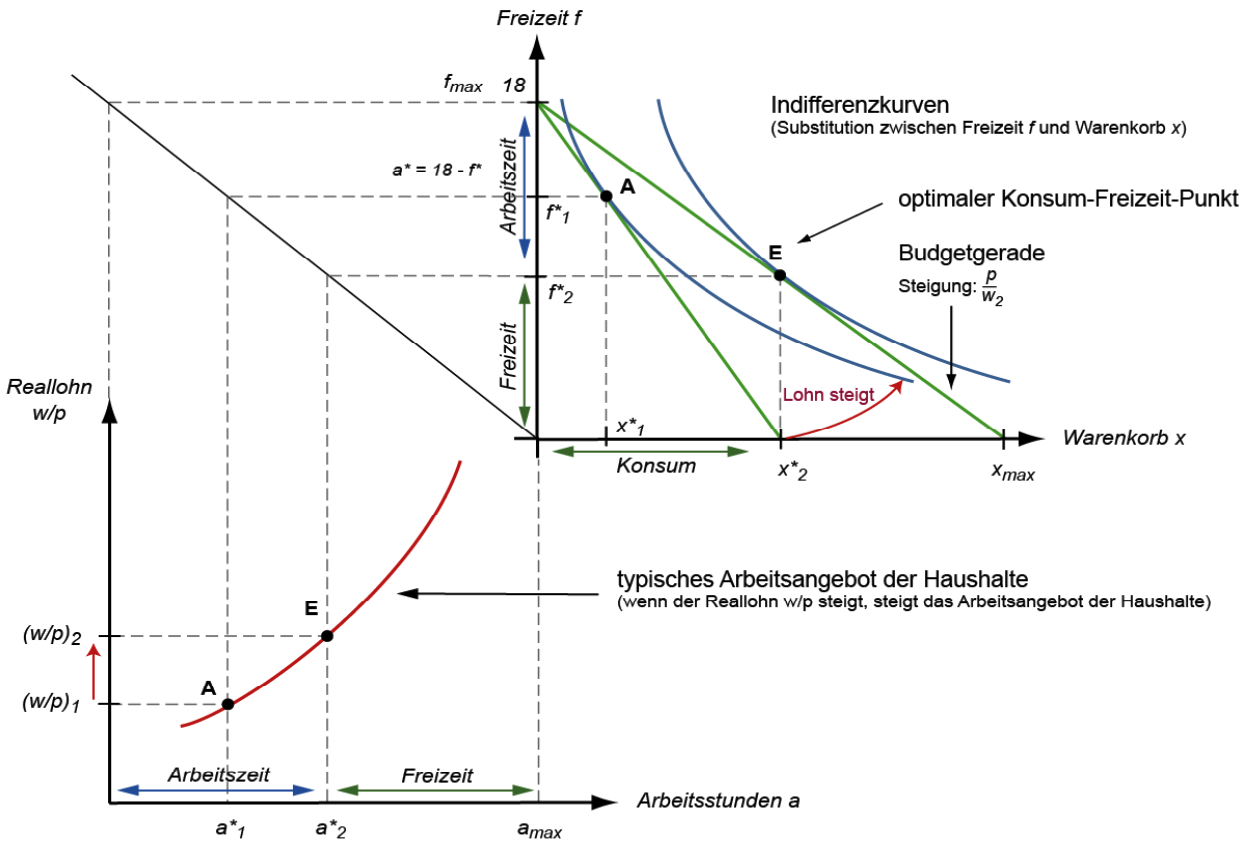
\includegraphics[width=8cm]{Arbeitsangebot_2.png}
\end{center}

Sobald sich der Lohn erhöht, dann sinkt einerseits die Steigung der Budgetgerade. Es entsteht ein neues Optimum, wobei die Freizeit sinkt und die Arbeitszeit steigt. \newline

\textbf{Empirische Daten} zeigen auf, dass die Kurve des Arbeitsangebots der Haushalte nicht undendlich lange steigt. Am einem gewissen Punkt ($a^*, (w/p)^*$) kommt es zu einer Umkehr/ einem Wendepunkt und die Arbeit nimmt als Funktion des Lohnes wieder ab. Die Freizeit wird ab einem gewissen Punkt höher gewertet als der Konsum. \newline

\textbf{Lohnelastizität} des Arbeitsangebotes der Haushalte gibt an, um wieviel Prozent sich die angebotene Arbeitsleistung der Haushalte ändert, wenn der Lohnsatz pro Stunde um ein Prozent verändert wird.

\begin{equation}
    \varepsilon_{a,w} = \frac{\partial a^{\text{Angebot}}}{\partial w} \frac{w}{a^{\text{Angebot}}}
\end{equation}

Im steigenden Teil der Arbeitsangebotsfunktion ist die Elastizität positiv, im fallenden Teil negativ.

\subsubsection{Arbeitsnachfrage}

Die Arbeitgeber fragen nach Arbeit nach, wobei sie im freien Markt gewinnmaximierend operieren möchten:

\begin{align}
    G(x) = E(x) - K(x) = \overline{p} x(a) - K(x(a))
\end{align}

Der Preis ist konstant und wird durch den Markt vorgegeben. Die produzierte Menge $x$ ist abhängig von der eingesetzten Arbeitsmenge $a$, und Faktoren $r$ natürliche Ressourcen und $k$ Sachkapital ($x = f(a,r,k)$). WIr nehmen nun zudem an, dass die Arbeitsmenge der Arbeitnehmer ebenfalls vorgegeben ist $\overline{W}$:

\begin{equation}
    G(a) = \overline{p} f(a) - \overline{w} a
\end{equation}

Die notwendige Bedinung für Gewinnmaximierung:

\begin{align}
    G'(a) = 0 = \overline{p} f'(a) - \overline{w} \\
    f'(a) = \frac{\overline{w}}{\overline{p}} \\
    \text{Grenzproduktivität der Arbeit} = \text{Reallohn}
\end{align}

Für die hinreichende Bedingung gilt immer, dass die Grenzproduktivität abnimmt: 

\begin{align}
    G''(a) = \overline{p}f''(a) < 0 \Leftrightarrow f''(a) < 0
\end{align}

Die \textbf{Grenzproduktivität} der Arbeit ist der zusätzliche Output, der aus dem Einsatz einer zusätzlichen Einheit Arbeit resultiert.

\begin{center}
    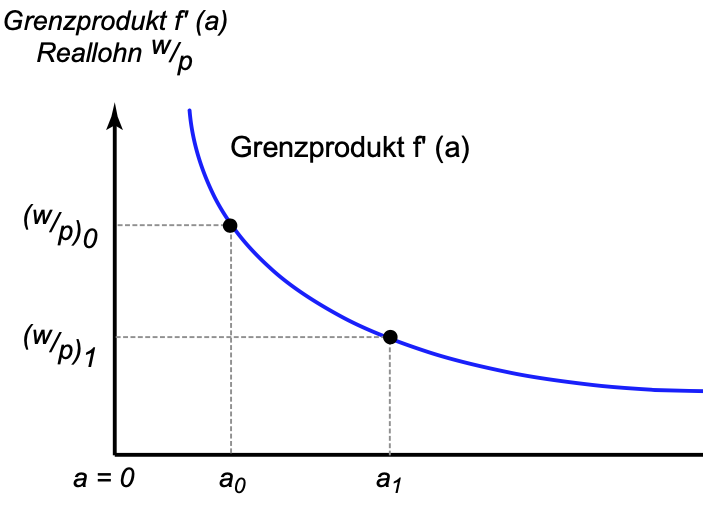
\includegraphics[width=8cm]{Grenzprodukt.png}
\end{center}

Die Arbeitsnachfragekurve des einzelnen Unternehmens entspricht der Grenzproduktivitätskurve. Bei einem Reallohn $(w/p)_0$ fragt das Unternehmen eine Arbeitsleistung von $a_0$ nach. Mit sinkendem Reallohn $(w/p)_1$ ist der Unternehmer bereit mehr Arbeit $a_1$ nachzufragen.


\begin{align}
    f'(a)\cdot \overline{p} = \overline{w} \\
    \text{Grenzwertprodukt der Arbeit} = \text{Nominallohn}
\end{align}

Das \textbf{Grenzwertprodukt} ist der zusätzliche bewertete Output (zusätzlicher Erlös), der daraus resultiert, dass eine Einheit Arbeit mehr eingesetzt wird. (Aus den vorherigen Gleichungen)

\subsubsection{Typen von Arbeitslosigkeit}

\textbf{Die Freiwillige Arbeitslosigkeit}: 

\begin{itemize}
    \item Idee: Mehr Arbeitskräftepotential ist grösser als Arbeitsmenge im Gleichgewicht 
    \item Alle, die bereit sind, für Lohn $w^*$ zu arbeiten, haben Arbeit 
    \item Diejenigen, die nicht bereit sind für Lohn $w^*$ zu arbeiten, haben keine Arbeit 
\end{itemize}

\begin{center}
    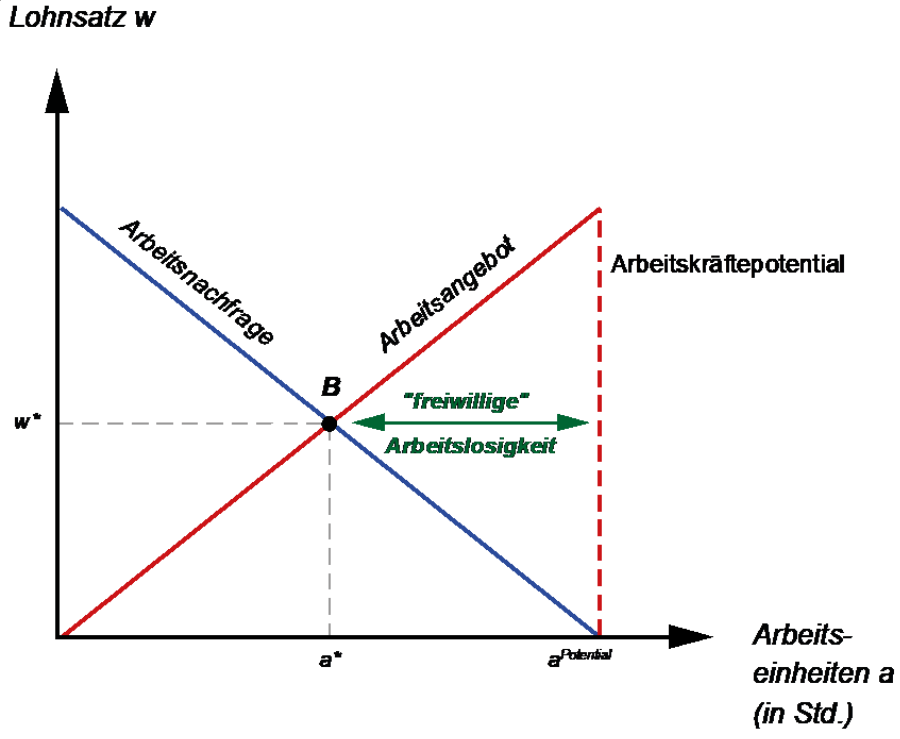
\includegraphics[width=8cm]{Freiwillige_Arbeitslosigkeit.png}
\end{center}

\textbf{Die Unfreiwillige Arbeitslosigkeit}:

\begin{itemize}
    \item Idee: Der tatsächliche Lohnsatz ist höher als der Gleichgewichts-Lohnsatz
    \item Nicht alle, die bereit sind, zum Lohnsatz $w_1$ zu arbeiten, finden auch Arbeit.
\end{itemize}

\begin{center}
    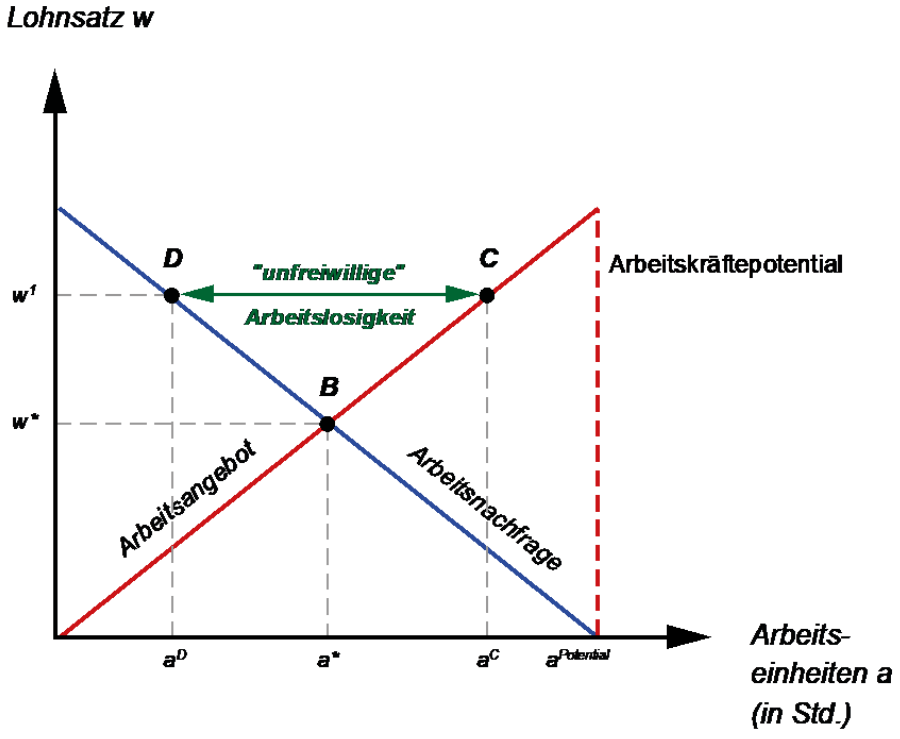
\includegraphics[width=8cm]{Unfreiwillige_Arbeitslosigkeit.png}
\end{center}

Der tatsächliche Lohn, z.B. ein (gesetzlicher) Mindestlohn, ist höher als der gleichgewichtige Lohnsatz $w^*$; die nachgefragte Arbeitsmenge $a_D$ zum Lohnsatz $w_1$ ist kleiner als die angebotene Arbeitsmenge $a_C$ zum tatsächlichen Lohnsatz $w_1$. Die unfreiwillige Arbeitslosigkeit beträgt dann der Strecke $a_C-a_D$.

\subsubsection{Erklärung und Bekämpfung von unfreiwilliger Arbeitslosigkeit}

\begin{enumerate}
    \item Ausgehandelte Löhne bzw. Mindestlöhne sind zu hoch und bewegen sich nicht nach oben (Lohnstarrheit):
    \begin{itemize}
        \item ...weil Mindestlöhne für einen längeren Zeitraum fixiert sind
        \item ...Arbeitnehmervertreter stimmen Lohnsenkungen nicht zu 
        \item ...Arbeitgebervertreter möchten hochqualifizierte Leute, bieten darum höhere Löhne an 
    \end{itemize}
    Die Massnahme gegen Lohnstarrheit wäre die Senkung des Lohnes. Ist jedoch schwierig aufgrund der involvierten Parteien 
    \item Die Güternachfrage, darum auch die Arbeitsnachfrage ist gering (Weniger Jobs im Strassenbau, weniger möchten da arbeiten):
    \begin{itemize}
        \item Die Arbeitsnachfrage verschiebt sich nach links bei gleichem Lohn $w^*$ wird jedoch nur noch $a_D$ angeboten
        \item Es fehlen also $a-a_D$ Arbeiter/Arbeitseinheiten 
    \end{itemize}
    Die Massnahme gegen eine sinkende Güternachfrage wären Umschulungen und Weiterbildungen der Leute, dass sie sich in einem anderen Metier wiederfinden können
\end{enumerate}

\subsection{Arbeitsmarktpolitik}

Die unfreiwillige Arbeitslosigkeit lässt sich noch weiter aufspalten: \newline

\textbf{Die konjunkturelle Arbeitslosigkeit} ist eine Art von Arbeitslosigkeit, die konjunkurell bedingt ist (kurz- und mittelfristig). Beispiel wäre eine Firma, die während einer Rezession Mitarbeiter entlassen muss. Diese werden im nächsten Aufschwung wieder eingestellt, was die Problematik relativiert. Der Staat kann via Fiskalpolitik die Zinsen senken und so oder durch Bau von Infrastruktur kurzzeitig reagieren. Die Privaten können durch kleinere Zinsen die Investitionen intensivieren. Der Zins wird durch die Notenbank bestimmt. \newline 

\textbf{Sockelarbeitslosigkeit} ist unabhängig von der Konjunktur. Diese lässt sich aufteilen in friktionelle und strukturelle Arbeitslosigkeit teilen:  \newline

\textbf{Friktionelle Arbeitslosigkeit} entstammt aus dem Zeitbedarf, den Arbeitnehmende brauchen um von einem Arbeitsplatz in einen anderen überzugehen. Massnahmen hierzu sind Umschulungen, Unterstützung bei der Stellensuche, Bereitstellung von Information über freie Stellen \newline

\textbf{Strukturelle Arbeitslosigkeit} wird durch zwei Thesen hervorgerufen: 

\begin{itemize}
    \item \emph{Neoklassisch}: Zu hohe oder starre Löhne bzw. hohe Arbeitskosten. Lösung hierzu ist die Senkung oder Abschaffung von Mindestlöhnen oder Flexibilisierung der Arbeitsmarktvorschriften
    \item Konsequenz: Tiefere individuelle Entlohnung und sinkende Jobsicherheit aber insgesamt höher Beschäftigungsgrade 
    \item \emph{Keynesianische Perspektive}: Geringe Güternachfrage führt zu geringerer Arbeitsnachfrage und daraus Arbeitslosigkeit 
    \item Lösung: Expansive Fiskal- oder Geldpolitik
\end{itemize}

\section{Aussenwirtschaft}

\subsection{Zahlungsbilanz}

Zahlungsbilanz = Monetäre Werte aller wirtschaftlichen Transaktionen während eines Jahres zwischen Inländern und Ausländern. Sie umfasst nur Flussgrössen und keine Standgrössen und ist in de Sinn etwas anderes als eine klassische Bilanz. 

Die Zahlungsbilanz umfasst meherer Teilbilanzen: 

\begin{enumerate}
    \item Leistungsbilanz (LB)
    \item Vermögensübertragungbilanz (VB)
    \item Kapitalbilanz (KB)
    \item Statistische Differenz (SD)
\end{enumerate}

Es gilt: 

\begin{equation}
    LB + VB - KB + SD = 0
\end{equation}

Die Transaktionen werden immer durch eine doppelte Buchführung erfasst und müssen daher ausgeglichen sein, wobei VB und SD bei In- und Auslandtransaktionen eine kleinere Rolle spielen. \newline 

\textbf{Überschüsse an Teilbilanzen} und deren Konsequenzen, zum Beispiel durch einen Exportüberschuss, sind tendenziell nur vorübergehend, da sie Wechselkursveränderungen bewirken.Fehlt dieser Mechnismus, sind solche Überschusse dauerhaft (z.B. China mit fixem Wechselkurs). Die Konsequenzen für:

\begin{itemize}
    \item Überschuss-Länder: Vergrösserung der Geldmenge, mehr Arbeit, Investitionskosten und Gesamtnachfrage. Gefahr jedoch von Inflation. Die Aufwertung der heimischen Währung reduziert die Überschüsse
    \item Defizit-Länder: Umgekehrt wie bei Überschuss-Ländern. Sinkende Geldmenge, Anstieg der Zinsen, Beschäftigungsrückgang. Deflation kann dadurch ebenfalls entstehen. 
\end{itemize}

\subsection{Handel und Handelshemmnisse}

Gründe, warum Handel betrieben wird sind folgende:

\begin{enumerate}
    \item Unterschiedliche Verfügbarkeit 
    \item Preisunterschiede
    \begin{itemize}
        \item Produktionskostenunterschiede 
        \begin{itemize}
            \item Ausstattung mit Produktionsfaktoren unterschiedlich 
            \item Produktivität der Produktionsfaktoren unterschiedlich 
        \end{itemize}
        \item Präferenzunterschiede 
    \end{itemize}
\end{enumerate}

Die Folgen für den Handel kann anhand der Transformationskurve (mögliche Outputkombinationen der Gesellschaft) und den Indifferenzkurven (Substitutionsmöglichkeiten zweier Güter) dargestellt werden. Diese bleiben in der Gesellschaft mit Handel unverändert, jedoch Preisverhältnisse der Güter durch den Weltmarkt vorgegeben und dadurch vom Wohlfahrtsmaximum (Autarkie) verschieden. 

\begin{center}
    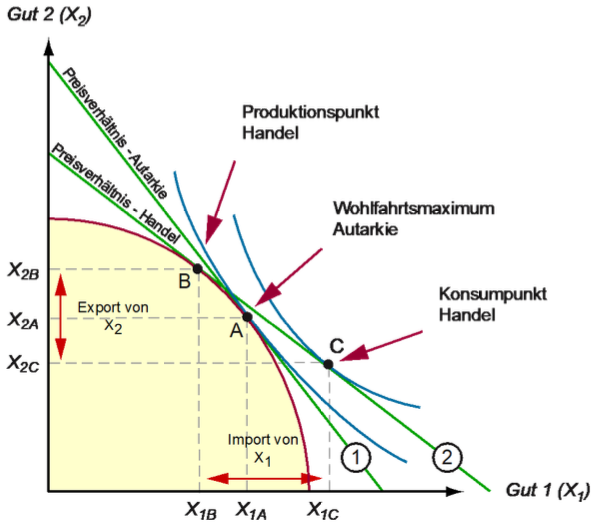
\includegraphics[width=8cm]{Wohlfahrtmaximum_Handel.png}
\end{center}

Nun kann sich durch den Import einer günstigeren Ware auf dem Weltmarkt $x_1$ und den Export von $x_2$ zu einer Verschiebung der Budgetgeraden führen, welche eine neue Nutzenniveau tangiert. Die Autarkie wird nun in zwei Punkte aufgespalten. Dem Produktionspunkt und dem Konsumpunkt. \newline

\textbf{Theorem der komparativen Kostenvorteile}: Es ist für ein Land vorteilhaft, nicht alle Güter, die von Inländern nachgefragt werden, selbst herzustellen. Das Land soll sich auf die Produktion jener Güter fokussieren, die möglichst günstig hergestellet werden können. \newline

\textbf{Bemerkungen zu Kostenvorteilen}: Aus statischer Perspektive wurde vorher gezeigt, dass Handel vorteilhaft ist. Aus dynamischer Sicht ist Handel vorteilhaft, wenn die Produktionsmöglichkeiten-Kurve (Transformationskurve) nach aussen verschoben wird. \newline

Handel kann Effekte verstärken. Es kommt nicht nur zu einem einmaligen Sprung im Sozialprodukt bzw. in der Wohlfahrt, sondern auch zu einem langfristigen Wachstum. \newline 

Wichtig ist es ebenfalls, dass Kostenvorteile ausgeglichen werden können (nicht, dass nur ein Land Vorteile hat). Eine Umstrukturierung der heimischen Wirtschaft benötigt Zeit und Transaktionskosten, die von Lobbygruppen (mit kurzsichtigen Intention) beklagt werden. Handelshemmnisse verhindern oft die Produktion ins Ausland. \newline 

\textbf{Handelshemmnisse} lassen sich in:

\begin{itemize}
    \item Tarifäre Handelshemmnisse, z.B Zölle 
    \item Nicht-tarifäre Handelshemmnisse, z.B. Importrestriktionen, techn. Vorschriften
\end{itemize}

aufteilen. Für einen autarken Markt mit GLeichgewichtspreis $p^*$ und -menge $x^*$ kann der Preis auf dem Weltmarkt $p_{Welt}$, mit zugehöriger Nachfrage $x_1^N$ bei mittels Zöllen erhöht werden. Die Nachfrage geht zurück und die angebotene Menge $x_2^A$ werden dann im Inland konsumiert und die Differenz importiert. Zölle haben jedoch Wohlfahrtsverluste zur Folge, da die Wohlfahrtsvorteile des freien Handels nicht (voll) zum Tragen kommen.


\begin{center}
    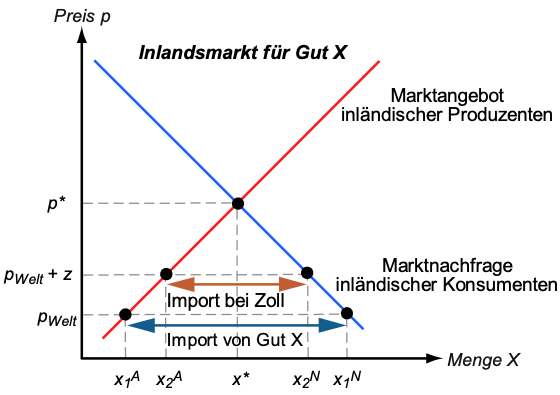
\includegraphics[width=8cm]{Importzoll.png}
\end{center}

\subsection{Bestimmung von Wechselkursen}

\textbf{Nominaler Wechselkurs} ist das Verhältnis, zu dem die Währung eines Landes gegen die Währung eines anderen Landes getauscht werden kann. \newline 

\textbf{Preisnotierung (Devisenkurs)}: Wieviel CHF entsprechen einer ausländischen Geldeinheit? Gegeben 1 einer Auslandwährung $\rightarrow$ wieviel CHF?\newline 

\textbf{Mengennotierung (Aussenwert)}: Wievel einer ausländischen Geldeinheit entsprechen einem CHF? Gegeben 1 CHF $\rightarrow$ wieviel einer Auslandwährung?

\begin{equation}
    \text{Preisnotierung} = \frac{1}{\text{Mengennotierung}}
\end{equation}

\textbf{Aufwertung}: Weniger CHF benötigt, um in ausländische Geldeinheit zu wechseln (Preisnotierung nach unten, Mengennotierung nach oben). Ausländische Wertung wird abgewertet \newline

\textbf{Abwertung}: Mehr CHF benötigt, um in ausländische Geldeinheit zu wechseln (Preisnotierung nach oben, Mengennotierung nach unten). Ausländische Wertung wird aufgewertet \newline 

\begin{center}
    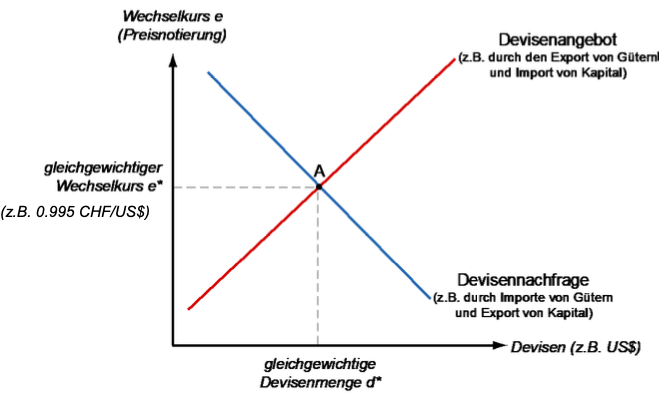
\includegraphics[width=8cm]{Bestimmung_nomineller_Wechselkurs.png}
\end{center}

Der nominale Wechselkurs wird durch dias Devisenangebot und die Devisennachfrage bestimmt. Der gleichgewichtige Wechselkurs liegt dort, wo Devisenangebot- und - nachfragemengen übereinstimmen. Wenn der Wechselkurs steigt, wird die inländische Währung abgewertet bzw. die ausländische Währung aufgewertet. Wenn der Wechselkurs sinkt, wird die inländische Währung aufgewertet bzw. die ausländische Währung abgewertet. Die Zentralbanken können das Devisenangebot wie auch die Devisennachfrage aktiv steuern\newline 

\textbf{Realer Wechselkurs}ist das Verhältnis, zu dem Waren und Dienstleistungen eines Landes gegen Waren und Dienstleistungen eines anderen Landes getauscht werden können.

\begin{equation}
    \text{Realer Wechselkurs} = \frac{\text{Nom. WK}\cdot \text{Ausländischer Preis des Warenkorbs}}{\text{Inländischer Preis des Warenkorbs}}
\end{equation}

Der reale Wechselkurs ist dimensionslos und bringt Kaufkraftunterschiede zwischen je zwei Ländern zum Ausdruck. \newline 

Der reale Wechselkurs ist dimensionslos und bringt Kaufkraftunterschiede zwischen je zwei Ländern zum Ausdruck. \newline

\textbf{Flexibles Wechselkurssystem}: Zentralbank und Regierung können einer Auf-/Abwertung mit
expansiver/restriktiver Geldpolitik entgegenwirken \newline 

\textbf{Fixes Wechselkurssystem}: Zentralbank muss bei Auf-/Abwertungen mit entsprechender Geldpolitik eingreifen, um den Wechselkurs aufrecht zu erhalten; die Geldpolitik ist damit nicht mehr autonom

\section{Geld}

\subsection{Funktionen des Geldes}

Funktionen des Geldes: 

\begin{enumerate}
    \item Tausch-/Zahlungsmittel: Bei Transaktionen, wichtig ist Akzeptanz (durch Vertrauen oder Gesetz)
    \item Recheneinheit: Massstab, mit dem wir ökonomische Transaktionen messen 
    \item Wertaufbewahrung: Kaufkraft kann auf zukünftige Perioden übertragen werden (Transaktionskosten sind extrem gering/praktisch null)
\end{enumerate}

Arten von Geld: 

\begin{enumerate}
    \item Bargeld: Noten + Münzen im Umlauf. Sind der liquidste Vermögenstitel 
    \item Buchgeld/Giralgeld: Einlagen auf Bankkonten oder Girokonten, die sofort liquidierbar sind (Geschäftsbankengeld) 
\end{enumerate}

\begin{center}
    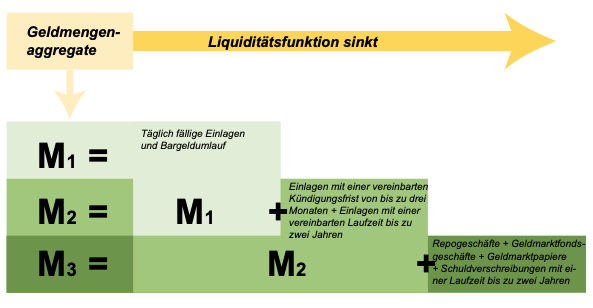
\includegraphics[width=8cm]{Geldmengenaggregate.png}
\end{center}

\begin{itemize}
    \item $M_1$: Tägliche Einlagen udn Bargeldumlauf (Bürger und Banken)
    \item $M_2$: Einlagen mit vereinbarten Kündigungsfrist + Einlagen mit einer vereinbarten Laufzeit bis zu zwei Jahren 
    \item $M_3$: Repogeschäfte + Geldmarktfondsgeschäfte + Geldmarktpapiere + Schuldverschreibungen mit einer Laufzeit von bis zu zwei Jahren 
\end{itemize}

\subsection{Geldschöpfung}

Ein grosser Teil des im Umlauf befindlichen Geldes entsteht durch einen anderen, durch die Notenbank nicht direkt zu kontrollierenden Prozess, den so genannten Geldschöpfungsprozess.

\begin{equation}
   \text{Geldschöpfungspotential}~ M_r = \underbrace{\frac{1}{r}}_{m_r}\cdot \text {Zentralbankgeld}
\end{equation}
\begin{equation}
    \text{Geldschöpfungspotential}:= \underbrace{\frac{1}{c+r(1-c)}}_{m_k}\cdot \text {Zentralbankgeld}
\end{equation}   

\begin{align}
    r := \text{Mindestreservesatz} \\
    c := \text{Kassenhaltungskoeffizient / KK} \\
    m_k := \text{Einfacher Geldschöpfungsmultipl.} \\
    m_r := \text{Geldschöpfungsmultiplikator mit KK} 
\end{align}

Der Mindestreservesatz ist der Anteil der Bankeinlagen, welcher von den Geschäftsbanken bei der Zentralbank hinterlegt werden muss. Je höher der Mindestreservesatz ist, desto geringer ist das Geldschöpfungspotential der Geschäftsbanken. \newline 

Die Geldschöpfung durch die Geschäftsbanken wird im Normalfall durch einen weiteren Faktor limitiert. In der Regel bringen die Kunden der Geschäftsbanken nämlich nicht die gesamte von ihnen gehaltene Geldmenge auf die Bank, sondern behalten einen bestimmten Anteil als Bargeld in der eigenen Kasse. Der durchschnittliche Anteil an gehaltenem Bargeld wird durch den sogenannten Kassenhaltungskoeffizienten (c) ausgedrückt.

\subsection{Geldpolitik und Geldpolitische Instrumente}

Hauptziele der meisten Nationalbanken:

\begin{enumerate}
    \item Preisstabilität = konstante, kontrollierte, eher tiefe Inflation (konstantes, moderates Preiswachstum)
    \item Stabilisierung der Konjunkturentwicklung: Stimulieren und Bremesen um BIP anzuheben (Rezession) oder zu bremsen (Boom)
\end{enumerate}

In gewissen Situationen kann es zu Konflikten kommen, zum Beispiel: 

\begin{itemize}
    \item Hohe Preise und niedrige wirtschaftliche Aktivität
    \item Man kann nur eines auf's mal angehen (Zinsen senken $\rightarrow$ wirtschaftliche Aktiviät erhöhen)
    \item Preise bleiben jedoch gleich. Man muss Prioritäten setzen 
\end{itemize}

\subsubsection{Geldpolitische Instrumente}

\begin{itemize}
    \item Geldmenge steuern 
    \item Zinsen steuern 
\end{itemize}

Die \textbf{Geldmenge} lässt sich durch M1, M2 und M3 zusammensetzen und lässt sich über die \emph{Offenmarktpolitik} steuern. Basis dieser Strategie ist die Festlegung der Zentralbankmenge. Somit kann direkt das Gelschöpfungspotential gesteuert werden. \newline 

Die \textbf{Zinsen} werden über den Mindestreservesatz, also den Prozentsatz der Einlagen bei den Geschäftsbanken $c$ oder den Reposatz. \newline 

Beim \textbf{Repogeschäft} verkauft die Geschäftsbank der Zentralbank Wertpapiere und Devisen gegen Notenbankgeld und bezahlt einen Zins. Die Geschäftsbank kauft sich nach einer vorbestimmten Zeit die Positionen zurück. Wenn die Geldmenge erhöht werden soll, wird der Reposatz verringert (die Banken werden als Reaktion mehr Postiionen verkaufen). \newline 

\emph{Da das Repogeschäft täglich lauft}, ist es einfacher über jenes das Notenbankgeld zu steuern als über den Mindestreservesatz. \newline

Die \textbf{Geldpolitik} lässt sich in zwei Typen einteilen:

\begin{itemize}
    \item Expansive Geldpolitik: Geldmenge bei Geschäftsbanken erhöhen 
    \begin{enumerate}
        \item Wirkungskette: Geschäftsbanken geben Kredite $\rightarrow$ Geldmenge in Volkswirtschaft steigt $\rightarrow$ mehr Transaktionen 
        \item Wirkungskette: Tiefe Zinsen $\rightarrow$ höhere Investitionen $\rightarrow$ gesamtwirtschaftliche Nachfrage steigt $\rightarrow$ Inflation möglich
    \end{enumerate}
    \item Restriktive/kontraktive Geldpolitik: Verkleinerung der Geldmenge bei Geschäftsbanken 
    \begin{enumerate}
        \item Weniger Kredite $\rightarrow$ weniger Geld im Kreislauf 
        \item Höhere Zinsen $\rightarrow$ weniger Investitionen 
    \end{enumerate}
\end{itemize}

\subsection{Definition, Messung und Bedeutung von Inflation}

\textbf{Inflation} ist die Bezeichnung für das Ansteigen des gesamtwirtschaftlichen allgemeinen Preisniveaus einer Volkswirtschaft über die Zeit

\begin{align}
    \text{Inflationsrate} := \frac{P_t - P_{t-1}}{P_{t-1}}\cdot 100\% \\
    P_t: \text{Preisniveau im laufenden Jahr t} \\
    P_{t-1}: \text{Preisniveau im Vorjahr}
\end{align}

Das Preisniveau wird durch einen Verbrauchskorb (Durchschnittspreise und Verbrauchmengen) eines Durchschnittshaushalts bestimmt für eine Referenzperiode (0) und später für eine andere Periode mit dem gleichen Warenkorb: 

\begin{align}
    P_0 = \frac{\sum_{i=1}^N p_{0i}\cdot q_{0i}}{\sum_{i=1}^N q_{0i}} \\
    \frac{P_t}{P_0} = \frac{\sum_i^N p_{ti}\cdot q_{0i}}{\sum_i^N p_{0i}\cdot q_{0i}} = \text{Laspeyres Index}\\
    \frac{P_t-P_{t-1}}{P_{t-1}} = \frac{\frac{P_t}{P_0}-\frac{P_{t-1}}{P_0}}{\frac{P_{t-1}}{P_0}} = \frac{\sum(p_{ti}-p_{ti-1})q_{0i}}{\sum p_{ti-1}\cdot q_{0i}}
\end{align}

\textbf{Unerwünschte Effekte von Inflation}:

\begin{itemize}
    \item \textbf{Unerwünschte Verteilungseffekte}
    \begin{itemize}
        \item Finanzielle Schuldner werden begünstigt, Gläubiger benachteiligt 
        \item Besitzer von Realvermögen werden begünstigt, Besitzer von Geldvermögen werden benachteiligt 
        \item Zahler fixierter Einkommen werden begünstigt, Empfänger fixierter Einkommen werden benachteiligt 
    \end{itemize}
    \item \textbf{Unerwünschte Produktionseffekte}
    \begin{itemize}
        \item Sparmotivation sinkt (Kreditzinsen erhöht durch die Bank als Reaktion)
        \item Mehr Spekulation (durch Unsicherheiten in Zukunft)
        \item Planungsunsicherheiten bei Unterehmen (bei hoher Inflation), reduziertes Investitionsvolumen
    \end{itemize}
\end{itemize}

\textbf{Fazit}: Inflation sollte reduziert werden, nur die negativen Folgen von Inflation zu vermindern. Wirtschaftspolitisch ist es das Ziel, ursachenadäquat zu handeln. \newline

\textbf{Deflation}: Negative Folgen sind für

\begin{itemize}
    \item Konsumenten: Käufe werden nach hinten verschoben in der Zeit. Nachfrage geht schnell zurück 
    \item Finanzmarkt: Der reale Zins steigt, ergo sinkende Investitionen 
\end{itemize}

\subsection{Ursachen und Bekämpfung von Inflation}

\textbf{Inflationsursachen}:

\begin{enumerate}
    \item Anstieg der gesamtwirtschaftlichen Nachfrage. Das Angebot wächst nicht mit der Nachfrage mit. Als Folge steigen die Preise 
    \item Von der Angebotsseite: 
    \begin{itemize}
        \item Anstieg der Produktionskosten 
        \item Anstieg der Gewinnmargen 
    \end{itemize}
\end{enumerate}

\textbf{Massnahmen} für Punkte 1 und 2:

\begin{enumerate}
    \item Inländische Nachfrage drosseln\dots
    \begin{itemize}
        \item durch Minderausgaben beim Staat
        \item durch höhere Besteuerung 
        \item Alternativ: Zinssenkung (benötigt jedoch Zeit und kann nur gewisse Effekte mildern)
    \end{itemize}
    \item Kostensteigerung und Margen im Rahmen zu halten z.B. durch Bündnis für Arbeit 
    \item (1+2) Drosselung der umlaufenden Menge via Zinsanstieg (oder Mindestreserve)
\end{enumerate}


\end{multicols*}
\end{document}